% Task C03
% Source volume: upper
% Physical scan pages: 84--113
% Printed book pages: 67--96
% Transcribe only source content; omit running headers, footers, and printed page numbers.
\chapter{实数系的基本定理}

% BEGIN TRANSCRIPTION

数列极限的基础是实数系的基本定理。在上一章中占有中心地位的单调有界数列的收敛定理就是其中之一。在本书中不讨论如何建立实数系，而是在下面分节介绍实数系的其他 5 个基本定理，包括以这些定理为基础的各种方法，以及它们在数列极限理论中的应用。在 §3.6 介绍上极限和下极限。本章中的许多内容都与数列极限有关，它们与第二章一起，给出了数列极限理论的比较完整的基本介绍。最后一节是学习要点和两组参考题。

\section{确界的概念和确界存在定理}

\subsection{基本内容}

这里最基本的概念、定义和定理如下（其中凡提到数集时均指非空实数集）：

\begin{enumerate}
  \item 一个实数集合有上界不一定有最大数，有下界不一定有最小数。
  \item 定义：(1) 如果 $A$ 是一个有上界的实数集，则称 $A$ 的最小上界为 $A$ 的上确界；(2) 如果 $A$ 是一个有下界的实数集，则称 $A$ 的最大下界为 $A$ 的下确界。
  \item 记号：数集 $A$ 的上确界记为 $\sup A$，数集 $A$ 的下确界记为 $\inf A$。
  \item 如果数集 $A$ 有最大数，则这个最大数就是 $A$ 的上确界；如果数集 $A$ 有最小数，则这个最小数就是 $A$ 的下确界。
  \item 确界存在定理：在实数系中，有上界的数集一定有上确界，有下界的数集一定有下确界。
  \item 对无上界的数集 $A$，约定 $\sup A=+\infty$；对无下界的数集 $A$，约定 $\inf A=-\infty$。
  \item 由上确界的定义知道：数 $\beta$ 是数集 $A$ 的上确界，如果满足以下两个条件：
  \begin{enumerate}[label=(\arabic*)]
    \item $\beta$ 是 $A$ 的上界，即对每一个数 $x\in A$，成立 $x\leqslant\beta$；
    \item 比 $\beta$ 小的数不会是数集 $A$ 的上界，即对每一个数 $\beta'<\beta$，存在 $x'\in A$，使得 $x'>\beta'$。
  \end{enumerate}
  \item 由下确界的定义知道：数 $\alpha$ 是数集 $A$ 的下确界，如果满足以下两个条件：
  \begin{enumerate}[label=(\arabic*)]
    \item $\alpha$ 是 $A$ 的下界，即对每一个数 $x\in A$，成立 $x\geqslant\alpha$；
    \item 比 $\alpha$ 大的数不会是数集 $A$ 的下界，即对每一个数 $\alpha'>\alpha$，存在 $x'\in A$，使得 $x'<\alpha'$。
  \end{enumerate}
  \item 数集的上（下）确界如果存在，则必定唯一。
\end{enumerate}

\subsection{例题}

由确界存在定理可以证明单调有界数列的收敛定理。初学者要注意在这个证明中对于单调数列的极限作出了准确的刻画。

\begin{xexample}[3.1.1]
用确界存在定理证明单调有界数列一定收敛。
\end{xexample}
\begin{xproof}
不妨只讨论单调减少的有界数列。设 $\{a_n\}$ 是一个这样的数列，即有
\[
  a_1\geqslant a_2\geqslant\cdots\geqslant a_n\geqslant\cdots,
\]
同时根据条件，这个数列有下界（它显然以 $a_1$ 为上界）。

现考虑数集 $A=\{a_n\mid n\in\NN_+\}$。由于数列有下界，因此数集 $A$ 有下界。对 $A$ 应用确界存在定理，知道 $A$ 有下确界，记这个下确界为 $a=\inf A$。

根据下确界的定义，$a$ 是数集 $A$ 的最大下界，因此一方面，对每个 $n$ 有 $a_n\geqslant a$。另一方面，对每一个 $\varepsilon>0$，比 $a$ 大的数 $a+\varepsilon$ 就不能再是数集 $A$ 的下界，因此在数列中一定有一项比 $a+\varepsilon$ 还要小，将这一项记为 $a_N$，就得到
\[
  a+\varepsilon>a_N.
\]
由于数列的单调减少性质，当 $n>N$ 时成立
\[
  a+\varepsilon>a_N\geqslant a_n\geqslant a.
\]
因此在 $n>N$ 时就得到
\[
  \abs{a_n-a}\leqslant\abs{a_N-a}<\varepsilon.
\]
这样就证明了单调减少有界数列收敛，而且它的极限就是数集 $A$ 的下确界。
\end{xproof}

必须强调指出，确界存在定理是在实数系 $\RR$ 中才成立的。

\begin{xexample}[3.1.2]
举例说明：有上界的有理数集在 $\QQ$ 中可以没有上确界，有下界的有理数集在 $\QQ$ 中可以没有下确界。
\end{xexample}
\begin{xsolution}
对两个论断之一举例就够了。从中学数学出发，将无理数理解为不循环十进无限小数，则只要取 $\sqrt2$ 的 $n$ 位有效不足近似值作为 $a_n$：$a_1=1$，$a_2=1.4$，$a_3=1.41,\cdots$，就得到严格单调增加的有理数数列 $\{a_n\}$，它收敛于 $\sqrt2$。从上一个例题可知，这也就是数集 $A=\{a_n\mid n\in\NN_+\}$ 的上确界。由于上确界唯一，因此数集 $A$ 在有理数集中就没有上确界。
\end{xsolution}

\begin{xremark}
由此可知：在有理数集 $\QQ$ 中的单调有界数列在 $\QQ$ 中可以没有极限。
\end{xremark}

下一个例题说明在确界和数列之间存在密切联系。

\begin{xexample}[3.1.3]
设 $A$ 是有上界的数集，$\beta=\sup A$。证明：存在 $\{a_n\}$，使 $a_n\in A$，$n\in\NN_+$，而且 $\lim_{n\to\infty}a_n=\beta$。又若 $\beta\notin A$，则 $\{a_n\}$ 可以是严格单调增加的。
\end{xexample}
\begin{xproof}
如果 $A$ 的上确界就是数集的最大数，即 $\beta=\sup A\in A$，则只要简单取 $a_n=\beta$（$n\in\NN_+$）即可。这时数列 $\{a_n\}$ 是常值数列。以下讨论 $\beta\notin A$ 的情况。

由于 $\beta$ 是数集 $A$ 的最小上界，对每个正整数 $n$，$\beta-1/n$ 不会是数集 $A$ 的上界。因此在 $A$ 中至少存在一个数比 $\beta-1/n$ 大，将它记为 $a_n$。对每个 $n$ 都这样做，就得到一个数列 $\{a_n\}$。从不等式
\[
  \beta-\frac1n<a_n\leqslant\beta,\qquad n\in\NN_+
\]
可见，数列 $\{a_n\}$ 收敛于 $\beta$。

为了使得数列 $\{a_n\}$ 严格单调增加（这同时使数列中的每一项和其他任何一项不相等），对以上的做法还要作一点改进。实际上，在取定第一项时，有 $\beta-1<a_1\leqslant\beta$。但由于 $\beta$ 不属于数集 $A$，因此它不会等于 $a_1$。这样就得到
\[
  \beta-1<a_1<\beta.
\]
由于 $a_1$ 和 $\beta-\frac12$ 都比 $\beta$ 小，即 $\max\{a_1,\beta-\frac12\}<\beta$，因此可以在数集 $A$ 找到 $a_2$，使它同时满足条件：
\[
  \beta-\frac12<a_2<\beta\quad\text{和}\quad a_1<a_2.
\]
注意：根据上述同样的理由，已将不等式 $a_2\leqslant\beta$ 改为 $a_2<\beta$。这样归纳地做下去，就可以取到数列 $\{a_n\}$，使得对每一个 $n$ 同时成立不等式
\[
  \beta-\frac1n<a_n<\beta\quad\text{和}\quad a_{n-1}<a_n.
\]
其中第一个不等式使 $\{a_n\}$ 收敛于 $\beta$，第二个不等式保证它严格单调增加。
\end{xproof}

\subsection{练习题}

\begin{xexercise}[1]
试证明确界的唯一性。
\end{xexercise}
\begin{xsolution}
先证上确界。设 $\alpha$ 与 $\beta$ 都是数集 $A$ 的上确界。因为 $\alpha$ 是最小上界，而 $\beta$ 是 $A$ 的一个上界，所以 $\alpha\leqslant\beta$；交换 $\alpha,\beta$ 的地位，又因 $\beta$ 是最小上界而 $\alpha$ 是上界，得 $\beta\leqslant\alpha$。故 $\alpha=\beta$。

再证下确界。若 $\gamma,\delta$ 都是 $A$ 的下确界，则 $\gamma$ 是最大下界而 $\delta$ 是一个下界，所以 $\gamma\geqslant\delta$；同时 $\delta$ 是最大下界而 $\gamma$ 是一个下界，所以 $\delta\geqslant\gamma$。因此 $\gamma=\delta$。故上下确界若存在都唯一。
\end{xsolution}


\begin{xexercise}[2]
设对每个 $x\in A$ 成立 $x<a$。问：在 $\sup A<a$ 和 $\sup A\leqslant a$ 中哪个是对的？
\end{xexercise}
\begin{xsolution}
必然成立的是
\[
  \sup A\leqslant a.
\]
因为 $x<a$ 对一切 $x\in A$ 成立，所以 $a$ 是 $A$ 的上界，最小上界不超过任一上界。

一般不能推出 $\sup A<a$。例如取 $A=(0,a)$（设 $a>0$），则对每个 $x\in A$ 都有 $x<a$，但 $\sup A=a$。
\end{xsolution}


\begin{xexercise}[3]
设数集 $A$ 以 $\beta$ 为上界，又有数列 $\{x_n\}\subset A$ 和 $\lim_{n\to\infty}x_n=\beta$。证明：$\beta=\sup A$。
\end{xexercise}
\begin{xsolution}
因为 $\beta$ 是 $A$ 的上界，只需证明任何小于 $\beta$ 的数都不是 $A$ 的上界。任取 $c<\beta$，令
\[
  \varepsilon=\frac{\beta-c}{2}>0.
\]
由 $x_n\to\beta$，存在 $N$，当 $n>N$ 时有
\[
  x_n>\beta-\varepsilon=\frac{\beta+c}{2}>c.
\]
而 $x_n\in A$，故 $c$ 不是 $A$ 的上界。于是 $\beta$ 是 $A$ 的最小上界，即 $\beta=\sup A$。
\end{xsolution}


\begin{xexercise}[4]
求下列数集的上确界和下确界：
  \begin{enumerate}[label=(\arabic*)]
    \item $\{x\in\QQ\mid x>0\}$；
    \item $\{y\mid y=x^2,\ x\in(-\frac12,1)\}$；
    \item $\{(1+\frac1n)^n\mid n\in\NN_+\}$；
    \item $\{n\ee^{-n}\mid n\in\NN_+\}$；
    \item $\{\arctan x\mid x\in(-\infty,+\infty)\}$；
    \item $\{(-1)^n+\frac1n(-1)^{n+1}\mid n\in\NN_+\}$；
    \item $\{1+n\sin\frac{n\pi}{2}\mid n\in\NN_+\}$。
  \end{enumerate}
\end{xexercise}
\begin{xsolution}
逐项计算如下。
\begin{enumerate}[label=(\arabic*)]
  \item 对 $A=\{x\in\QQ\mid x>0\}$，任意正实数都不是上界，故 $A$ 无上界；而 $0$ 是下界，且任意 $\alpha>0$ 都不是下界。因此
  \[
    \sup A=+\infty,\qquad \inf A=0.
  \]

  \item 当 $x\in(-\frac12,1)$ 时，$0\leqslant x^2<1$，且 $x=0$ 时取得 $0$；另一方面令 $x\to1^-$ 可使 $x^2$ 任意接近 $1$。故
  \[
    \inf\{x^2\mid x\in(-\tfrac12,1)\}=0,\qquad
    \sup\{x^2\mid x\in(-\tfrac12,1)\}=1.
  \]

  \item 记 $a_n=(1+1/n)^n$。由二项式展开
  \[
    a_n=\sum_{k=0}^{n}\frac1{k!}\prod_{j=0}^{k-1}\left(1-\frac{j}{n}\right).
  \]
  对每个固定的 $k\geqslant2$，乘积随 $n$ 增大而增大，且从 $n$ 到 $n+1$ 还增加一个正项，因此 $\{a_n\}$ 严格增加。又由已知基本极限 $a_n\to\ee$，故
  \[
    \inf\{a_n\}=a_1=2,
    \qquad
    \sup\{a_n\}=\ee.
  \]

  \item 令 $a_n=n\ee^{-n}>0$。有
  \[
    \frac{a_{n+1}}{a_n}=\left(1+\frac1n\right)\ee^{-1}<1,
  \]
  因为 $1+1/n\leqslant2<\ee$。故 $a_n$ 严格减少，而 $a_n\to0$。因此
  \[
    \sup\{n\ee^{-n}\}=\ee^{-1},\qquad
    \inf\{n\ee^{-n}\}=0.
  \]

  \item $\arctan x$ 在 $\RR$ 上取值于 $(-\pi/2,\pi/2)$，且当 $x\to\pm\infty$ 时分别趋于 $\pm\pi/2$。故
  \[
    \sup\{\arctan x\mid x\in\RR\}=\frac\pi2,
    \qquad
    \inf\{\arctan x\mid x\in\RR\}=-\frac\pi2.
  \]

  \item 令
  \[
    a_n=(-1)^n+\frac1n(-1)^{n+1}=(-1)^n\left(1-\frac1n\right).
  \]
  偶数项为 $1-1/n\to1$，奇数项为 $-1+1/n\to-1$，且所有项严格位于 $(-1,1)$ 内。因此
  \[
    \sup\{a_n\}=1,
    \qquad
    \inf\{a_n\}=-1.
  \]

  \item 对 $a_n=1+n\sin(n\pi/2)$，当 $n=4k+1$ 时 $a_n=1+n\to+\infty$；当 $n=4k+3$ 时 $a_n=1-n\to-\infty$。故
  \[
    \sup\{a_n\}=+\infty,
    \qquad
    \inf\{a_n\}=-\infty.
  \]
\end{enumerate}
\end{xsolution}


\begin{xexercise}[5]
证明：
  \begin{enumerate}[label=(\arabic*)]
    \item $\sup\{x_n+y_n\}\leqslant\sup\{x_n\}+\sup\{y_n\}$；
    \item $\inf\{x_n+y_n\}\geqslant\inf\{x_n\}+\inf\{y_n\}$。
  \end{enumerate}
\end{xexercise}
\begin{xsolution}
设有关确界均有意义。
\begin{enumerate}[label=(\arabic*)]
  \item 对每个 $n$，有
  \[
    x_n\leqslant\sup\{x_n\},\qquad
    y_n\leqslant\sup\{y_n\},
  \]
  因而
  \[
    x_n+y_n\leqslant\sup\{x_n\}+\sup\{y_n\}.
  \]
  右端是数集 $\{x_n+y_n\}$ 的上界，于是
  \[
    \sup\{x_n+y_n\}\leqslant\sup\{x_n\}+\sup\{y_n\}.
  \]

  \item 对下确界，由定义对每个 $n$ 有
  \[
    x_n+y_n\geqslant\inf\{x_n\}+\inf\{y_n\},
  \]
  故右端是 $\{x_n+y_n\}$ 的下界，从而
  \[
    \inf\{x_n+y_n\}\geqslant\inf\{x_n\}+\inf\{y_n\}.
  \]
\end{enumerate}
\end{xsolution}


\begin{xexercise}[6]
设有两个数集 $A$ 和 $B$，且对数集 $A$ 中的任何一个数 $x$ 和数集 $B$ 中的任何一个数 $y$ 成立不等式 $x<y$。证明：$\sup A\leqslant\inf B$。
\end{xexercise}
\begin{xsolution}
任取 $y_0\in B$，则 $y_0$ 是 $A$ 的上界，因此 $A$ 有上确界。任取 $x_0\in A$，则 $x_0$ 是 $B$ 的下界，因此 $B$ 有下确界。

对任意 $y\in B$，由于 $y$ 是 $A$ 的上界，有 $\sup A\leqslant y$。这说明 $\sup A$ 是 $B$ 的一个下界，故
\[
  \sup A\leqslant\inf B.
\]
\end{xsolution}


\begin{xexercise}[7]
设数集 $A$ 有上界，数集 $B=\{x+c\mid x\in A\}$，其中 $c$ 是一个常数。证明：
  \[
    \sup B=\sup A+c;\qquad \inf B=\inf A+c.
  \]
\end{xexercise}
\begin{xsolution}
先证上确界。记 $\alpha=\sup A$。对任意 $y\in B$，有 $y=x+c$，其中 $x\in A$，故
\[
  y=x+c\leqslant\alpha+c.
\]
所以 $\alpha+c$ 是 $B$ 的上界。另一方面，任取 $\varepsilon>0$，由上确界定义可取 $x\in A$ 使
\[
  x>\alpha-\varepsilon.
\]
于是 $x+c\in B$ 且
\[
  x+c>\alpha+c-\varepsilon.
\]
故任何小于 $\alpha+c$ 的数都不能作为 $B$ 的上界，所以
\[
  \sup B=\alpha+c=\sup A+c.
\]
对下确界，若 $\beta=\inf A$，则 $\beta+c$ 是 $B$ 的下界，并且对每个 $\varepsilon>0$ 可取 $x\in A$ 使 $x<\beta+\varepsilon$，从而 $x+c<\beta+c+\varepsilon$。故
\[
  \inf B=\inf A+c.
\]
上述结论在采用 $\pm\infty$ 约定时也按同样方式成立。
\end{xsolution}


\begin{xexercise}[8]
设 $A,B$ 是两个有上界的数集，又有数集 $C\subset\{x+y\mid x\in A,y\in B\}$，则 $\sup C\leqslant\sup A+\sup B$。举出成立严格不等号的例子。
\end{xexercise}
\begin{xsolution}
记 $\alpha=\sup A$，$\beta=\sup B$。若 $c\in C$，则存在 $x\in A,y\in B$ 使 $c=x+y$，于是
\[
  c=x+y\leqslant\alpha+\beta.
\]
故 $\alpha+\beta$ 是 $C$ 的上界，因此
\[
  \sup C\leqslant\sup A+\sup B.
\]
严格不等号例如取 $A=B=(0,1)$，$C=\{1\}$。此时
\[
  \sup C=1<2=\sup A+\sup B.
\]
\end{xsolution}


\begin{xexercise}[9]
设 $A,B$ 是两个有上界的数集，又有数集 $C\supset\{x+y\mid x\in A,y\in B\}$，则 $\sup C\geqslant\sup A+\sup B$。举出成立严格不等号的例子。
\end{xexercise}
\begin{xsolution}
仍记 $\alpha=\sup A$，$\beta=\sup B$。先证明
\[
  \sup\{x+y\mid x\in A,y\in B\}=\alpha+\beta.
\]
上界方向由上一题的论证立即得到。反之，任取 $\varepsilon>0$，可取 $x\in A,y\in B$ 使
\[
  x>\alpha-\frac\varepsilon2,
  \qquad
  y>\beta-\frac\varepsilon2.
\]
于是
\[
  x+y>\alpha+\beta-\varepsilon,
\]
故该和集的上确界不小于 $\alpha+\beta$。因此二者相等。

由于和集包含于 $C$，有
\[
  \sup C\geqslant\alpha+\beta.
\]
严格不等号例如取 $A=B=\{0\}$，$C=\{0,1\}$，则
\[
  \sup C=1>0=\sup A+\sup B.
\]
\end{xsolution}


（合并以上两题可见：当且仅当 $C=\{x+y\mid x\in A,y\in B\}$ 时成立 $\sup C=\sup A+\sup B$。）

\section{闭区间套定理}

\subsection{基本内容}

\begin{enumerate}
  \item 称 $\{I_n\}$ 为一个闭区间套，如果每个 $I_n$ 是闭区间，而且成立单调减少的包含关系，即 $I_n\supset I_{n+1}$，$n\in\NN_+$。也就是说有 $I_1\supset I_2\supset\cdots\supset I_n\supset\cdots$。
  \item 闭区间套定理：若 $\{I_n\}$ 为闭区间套，则 $\bigcap_{n=1}^{\infty}I_n\neq\varnothing$。又如 $I_n$ 的长度 $\abs{I_n}\to0$，则 $\bigcap_{n=1}^{\infty}I_n$ 为单点集。
  \item 闭区间套定理的另一种形式：设有闭区间序列 $\{[a_n,b_n]\}$ 满足条件
  \[
    a_n\leqslant a_{n+1}\leqslant b_{n+1}\leqslant b_n,\quad n\in\NN_+,
  \]
  则存在 $\xi$，使得 $a_n\leqslant\xi\leqslant b_n$，$n\in\NN_+$。又如 $\lim\abs{b_n-a_n}=0$，则上述 $\xi$ 是唯一的，这时数列 $\{a_n\}$ 和 $\{b_n\}$ 从点 $\xi$ 的两侧单调收敛于同一极限 $\xi$。
  \item 闭区间套定理的证明：从定理的第二种形式，就可以清楚地看出，闭区间套的左右端点分别形成两个数列，其中左端点所成的数列 $\{a_n\}$ 单调增加，以每个 $b_n$ 为上界；而右端点所成的数列 $\{b_n\}$ 单调减少，以每个 $a_n$ 为下界，因此它们都收敛。记 $\{a_n\}$ 的极限为 $\alpha$，$\{b_n\}$ 的极限为 $\beta$。在不等式 $a_n\leqslant b_n$ 两边取极限，就有 $\alpha\leqslant\beta$。而且对每个 $n$ 成立 $a_n\leqslant\alpha\leqslant\beta\leqslant b_n$。因此在 $\alpha$ 和 $\beta$ 之间取 $\xi$ 即可。在 $\abs{b_n-a_n}\to0$ 时，从推导可见 $\alpha=\beta$，因此 $\xi$ 唯一。
  \item \textbf{评注}\quad 从表面上看，与单调有界数列的收敛定理相比较，闭区间套定理似乎没有多少新的东西。后者只不过是含有两个有一定关系的单调数列而已。但实际上并非如此。这里可以指出两点：(1) 闭区间套定理并不限于实数系，可以推广为非常一般的形式，有许多重要应用，而单调性定理则离不开数直线上的序关系；(2) 与闭区间套定理相联系，有构造闭区间套的方法，从而在应用中往往要比单调有界数列的收敛定理强得多（见下面的例子）。
  \item 在上一章中已经见到许多例题，在其中有收敛于同一极限的两个单调性相反的单调序列。可以说在这些例题中自然地出现了闭区间套（请看第二章的例题 2.3.5，2.6.2，2.7.3 和命题 2.5.1 的证 1、命题 2.5.6，2.6.2 等）。
\end{enumerate}

\subsection{例题}

\begin{xexample}[3.2.1]
用闭区间套定理证明实数集 $\RR$ 是不可列集。
\end{xexample}
\begin{xproof}
用反证法。设 $\RR$ 可列，则存在 $\RR$ 与正整数集 $\NN_+$ 之间的一一对应，因此可以将实数集 $\RR$ 的所有元，即所有实数，排成一个序列：
\[
  \RR=\{x_1,x_2,\cdots,x_n,\cdots\}.
\]
现在开始构造闭区间套。根据 $x_1$，取闭区间 $I_1\subset\RR-\{x_1\}$，然后根据 $I_1$ 和 $x_2$，取闭区间 $I_2\subset I_1-\{x_2\}$。一般地，在有了 $I_{n-1}$ 之后，可以根据 $x_n$，取闭区间 $I_n\subset I_{n-1}-\{x_n\}$。这样就可以归纳地得到一个闭区间套 $\{I_n\}$。应用闭区间套定理，存在一个实数 $\xi$，它属于每一个闭区间 $I_n$，因此对每一个 $n$，都有 $\xi\neq x_n$。这样就找到了一个不在 $\RR$ 中的实数，引出矛盾。
\end{xproof}

现在通过例子介绍用 Bolzano（波尔查诺）二分法来构造闭区间套。

\begin{xexample}[3.2.2]
用闭区间套定理证明：有界数列必有收敛子列（即凝聚定理）。
\end{xexample}
\begin{xproof}
设 $\{x_n\}$ 有界，且有 $a<b$ 使 $a\leqslant x_n\leqslant b$ 对每个 $n$ 成立。改记 $a_1=a$，$b_1=b$，令 $I_1=[a_1,b_1]$ 为第一个闭区间，然后取这个区间的中点 $c_1=(a_1+b_1)/2$，这样得到两个子区间：$[a_1,c_1]$ 和 $[c_1,b_1]$。可以看出，在这两个子区间中至少有一个含有数列 $\{x_n\}$ 中的无穷多项。取具有这个性质的一个子区间为 $I_2$，记为 $[a_2,b_2]$。（如果两个子区间都有此性质，则任意取定一个为 $I_2$。）然后取 $I_2$ 的中点 $c_2=(a_2+b_2)/2$，同样在两个子区间 $[a_2,c_2]$ 和 $[c_2,b_2]$ 中取定一个记为 $I_3=[a_3,b_3]$，它含有数列 $\{x_n\}$ 中的无穷多项。这样进行下去，就可以归纳地得到一个闭区间套 $\{[a_n,b_n]\}$。在这里重要的是，它不仅是一个闭区间套，而且还具有构造过程所确定的两个特殊性质：(1) 从第二个闭区间起，每个闭区间的长度是前一个闭区间的长度的一半，也就是说有 $\abs{I_{n+1}}=\frac12\abs{I_n}$，$n\in\NN_+$；(2) 在每个闭区间中含有数列 $\{x_n\}$ 中的无穷多项。

应用闭区间套定理于上述 $\{I_n\}$，存在（唯一）$\xi\in\bigcap_{n=1}^{\infty}I_n$。但到此为止似乎与我们的目的还是毫不相干。（记住：我们的目的是要找一个收敛子列。）从闭区间 $I_1$ 中任取 $x_{n_1}$（当然可取 $n_1=1$），而在 $I_2$ 中由于它含有数列 $\{x_n\}$ 中的无穷多项，这就保证能在 $I_2$ 中取到 $x_{n_2}$，满足条件 $n_2>n_1$。这样归纳地做下去，就得到一个子列 $\{x_{n_k}\}$。它具有性质：$x_{n_k}\in I_k$，$k\in\NN_+$。由于
\[
  \abs{x_{n_k}-\xi}\leqslant\abs{I_k}=\frac1{2^{k-1}}\abs{I_1}=\frac1{2^{k-1}}(b-a),
\]
可见这个子列收敛于 $\xi$。
\end{xproof}

\begin{xremark}
请初学者重视上面这个例题，因为其中所用的构造闭区间套的方法具有典型意义。使用二分法必然具有性质 (1)，这保证了点 $\xi$ 唯一，但是更为重要的是构造出具有特殊性质 (2) 的闭区间套。
\end{xremark}

容易理解，对于每个具体问题，所构造的闭区间套一定要具有某种特殊性质。在上面的例题中，就是要求每个 $[a_n,b_n]$ 必须含有数列 $\{x_n\}$ 中的无穷多项。构造过程就是要求将这个性质保持下去。通过闭区间套定理将这个特性“凝聚”到一个点 $\xi$，也就是说在 $\xi$ 的任何一个邻域内都含有数列 $\{x_n\}$ 中的无穷多项。

为什么要使得这里的每个闭区间 $[a_n,b_n]$ 具有这个性质而不是别的什么性质？这完全由我们的目的所决定。我们的目的是选出收敛子列。由于用二分法得到的闭区间套收缩到唯一的点 $\xi$，因此只要从第 $k$ 个区间 $[a_k,b_k]$ 中选子列的第 $k$ 项，就保证了子列收敛。于是问题成为有否可能按这样的方式选出子列？

设想一下，如果已经有了子列的前 $k$ 项：$x_{n_1},\cdots,x_{n_k}$，它们的下标满足条件 $n_1<n_2<\cdots<n_k$。为了在区间 $[a_{k+1},b_{k+1}]$ 内能找到子列的下一项，即将数列的某一项选为 $x_{n_{k+1}}$，满足 $n_k<n_{k+1}$，当然需要在这个区间内有数列中的无穷多项以供选择。

以上考虑决定了在二分法中从两个子区间中究竟应当决定取哪一个。当然也许两个子区间都可以，这时任取一个即可。但一般而言是不能任取的。这方面的具体例子是下一小节的第一个练习题。

请初学者检查本书下面应用闭区间套定理的所有例子（也包括例题 3.2.1），观察在每个例子中构造闭区间套时的基本思想是否与这里所讲的相同。

\paragraph{小结}
在用闭区间套定理证明某个结论时，关键是如何构造闭区间套。具体而言，就是要确定该闭区间套应该具有什么样的特性。构造过程应该使这种特性从第一个闭区间开始“传递”给第二个闭区间，再从第二个闭区间“传递”给第三个闭区间，依次类推，直到将这个特性“凝聚”到闭区间套所共有的点的任意邻近。当然这种特性要能解决我们的问题。想清楚之后（而不是之前）就可以试写出证明。如果还是证明不出，说明上面的特性选择错了，从头再来。

\subsection{练习题}

\begin{xexercise}[1]
如果数列是 $\{(-1)^n\}$，开始的区间是 $[-1,1]$，试用例题 3.2.2 中的方法具体找出一个闭区间套和相应的收敛子列。又问：你能否用这样的方法在这个例子中找出 3 个收敛子列？
\end{xexercise}
\begin{xsolution}
从 $I_1=[-1,1]$ 出发，二分后选择含有无穷多个数列项 $1$ 的右半区间，得到
\[
  I_2=[0,1],\quad I_3=[1/2,1],\quad I_4=[3/4,1],\ \ldots
\]
即对 $k\geqslant2$ 可取
\[
  I_k=[1-2^{2-k},1].
\]
每个 $I_k$ 都含有无穷多个偶数项 $x_{2m}=1$，而 $\abs{I_k}\to0$，交集为 $\{1\}$。在 $I_k$ 中依次选取下标递增的偶数项，例如取 $x_{2k}=1$，便得到收敛子列 $x_{2k}\to1$。

可以用同样方法得到三个不同的收敛子列。例如
\[
  \{x_{2k}\},\qquad \{x_{4k}\},\qquad \{x_{4k+2}\}
\]
都恒等于 $1$，因而都收敛于 $1$。也可在第一步选择左半区间构造收敛于 $-1$ 的奇数项子列。
\end{xsolution}


\begin{xexercise}[2]
如闭区间套定理中的闭区间套改为开区间套 $\{(a_n,b_n)\}$，其他条件不变，则可以举出例子说明结论不成立。
\end{xexercise}
\begin{xsolution}
取
\[
  I_n=(0,1/n),\qquad n\in\NN_+.
\]
则 $I_{n+1}\subset I_n$，并且 $\abs{I_n}=1/n\to0$，但
\[
  \bigcap_{n=1}^{\infty}(0,1/n)=\varnothing.
\]
因为若 $x$ 属于所有这些区间，则 $x>0$，但取 $n>1/x$ 就有 $1/n<x$，矛盾。
\end{xsolution}


\begin{xexercise}[3]
如 $\{(a_n,b_n)\}$ 为开区间套，数列 $\{a_n\}$ 严格单调增加，数列 $\{b_n\}$ 严格单调减少，又满足条件 $a_n<b_n$，$n\in\NN_+$，证明 $\bigcap_{n=1}^{\infty}(a_n,b_n)\neq\varnothing$。
\end{xexercise}
\begin{xsolution}
由包含关系，$\{a_n\}$ 单调增加并以任一 $b_m$ 为上界；$\{b_n\}$ 单调减少并以任一 $a_m$ 为下界。因此存在有限极限
\[
  \alpha=\lim_{n\to\infty}a_n,
  \qquad
  \beta=\lim_{n\to\infty}b_n,
\]
且由 $a_n<b_n$ 得 $\alpha\leqslant\beta$。

严格单调性给出对每个 $n$ 都有
\[
  a_n<\alpha,\qquad \beta<b_n.
\]
取
\[
  \xi=\frac{\alpha+\beta}{2}.
\]
则对每个 $n$，
\[
  a_n<\alpha\leqslant\xi\leqslant\beta<b_n,
\]
故 $\xi\in(a_n,b_n)$ 对所有 $n$ 成立。因此
\[
  \bigcap_{n=1}^{\infty}(a_n,b_n)\neq\varnothing.
\]
\end{xsolution}


\begin{xexercise}[4]
用闭区间套定理证明确界存在定理。
\end{xexercise}
\begin{xsolution}
只证有上界的非空数集 $A$ 有上确界。任取 $u_1\in A$。若 $u_1$ 已是 $A$ 的上界，则 $u_1=\max A=\sup A$。否则取 $v_1$ 为 $A$ 的一个上界，于是 $u_1<v_1$，并且 $u_1$ 不是上界、$v_1$ 是上界。

对区间 $[u_n,v_n]$ 二分，令 $c_n=(u_n+v_n)/2$。若 $c_n$ 是 $A$ 的上界，置
\[
  u_{n+1}=u_n,\qquad v_{n+1}=c_n;
\]
若 $c_n$ 不是 $A$ 的上界，置
\[
  u_{n+1}=c_n,\qquad v_{n+1}=v_n.
\]
于是 $\{[u_n,v_n]\}$ 是闭区间套，且始终保持
\[
  u_n\text{ 不是 }A\text{ 的上界},\qquad v_n\text{ 是 }A\text{ 的上界},
\]
并有
\[
  v_n-u_n=2^{1-n}(v_1-u_1)\to0.
\]
由闭区间套定理，存在唯一 $\xi$ 使 $u_n\to\xi$、$v_n\to\xi$。

任取 $x\in A$。因每个 $v_n$ 都是上界，$x\leqslant v_n$，令 $n\to\infty$ 得 $x\leqslant\xi$，故 $\xi$ 是 $A$ 的上界。另一方面，若 $y<\xi$，则因 $u_n\to\xi$，可取 $n$ 使 $u_n>y$。由于 $u_n$ 不是 $A$ 的上界，存在 $x\in A$ 使 $x>u_n>y$，故 $y$ 不是上界。因此 $\xi$ 是最小上界，即 $\xi=\sup A$。

对下确界应用同样构造，或对集合 $-A$ 使用上确界结论，即得下确界存在定理。
\end{xsolution}


\begin{xexercise}[5]
用闭区间套定理证明单调有界数列的收敛定理。
\end{xexercise}
\begin{xsolution}
只讨论单调增加且有上界的情形。若 $a_1$ 已是数集
\[
  A=\{a_n\mid n\in\NN_+\}
\]
的上界，则由单调性有 $a_n=a_1$，结论成立。以下设 $a_1$ 不是 $A$ 的上界，并取 $A$ 的一个上界 $b_1>a_1$。

从闭区间 $I_1=[a_1,b_1]$ 开始二分。一般地，设已经得到
\[
  I_n=[u_n,v_n],
\]
其中 $u_n$ 不是 $A$ 的上界，而 $v_n$ 是 $A$ 的上界。令 $c_n=(u_n+v_n)/2$。若 $c_n$ 是 $A$ 的上界，取
\[
  I_{n+1}=[u_n,c_n];
\]
若 $c_n$ 不是 $A$ 的上界，取
\[
  I_{n+1}=[c_n,v_n].
\]
这样得到闭区间套 $\{I_n\}$，并且始终保持左端点不是 $A$ 的上界、右端点是 $A$ 的上界，同时
\[
  \abs{I_n}=2^{1-n}\abs{I_1}\to0.
\]
由闭区间套定理，存在唯一的 $\xi$ 使
\[
  u_n\to\xi,\qquad v_n\to\xi.
\]

任取 $\varepsilon>0$。取 $k$ 充分大，使
\[
  \xi-\varepsilon<u_k\leqslant\xi\leqslant v_k<\xi+\varepsilon.
\]
由于 $u_k$ 不是 $A$ 的上界，存在某个 $N$ 使 $a_N>u_k$；而 $v_k$ 是 $A$ 的上界，所以 $a_n\leqslant v_k$ 对所有 $n$ 成立。于是当 $n\geqslant N$ 时，由单调性得到
\[
  \xi-\varepsilon<u_k<a_N\leqslant a_n\leqslant v_k<\xi+\varepsilon.
\]
故 $a_n\to\xi$。

若 $\{a_n\}$ 单调减少且有下界，则对数列 $\{-a_n\}$ 应用刚才的结论，即得 $\{a_n\}$ 收敛。
\end{xsolution}


\section{凝聚定理}

\subsection{基本内容}

\begin{enumerate}
  \item 凝聚定理（Bolzano-Weierstrass（魏尔斯特拉斯）定理）：有界数列必有收敛子列。
  \item 凝聚定理在实数系中成立，在有理数集 $\QQ$ 中不成立（作为思考题）。
  \item \textbf{评注}\quad 从数列的极限理论知道，收敛数列一定有界，但有界数列不一定收敛。在一系列需要构造收敛数列的分析问题中，往往采取分两步走的方法，即一开始构造一个有界数列，然后对它用凝聚定理得到收敛子列。凝聚定理的这种用法往往有效，用形象化的语言来说，即是从混乱中找出了秩序。
\end{enumerate}

\subsection{例题}

凝聚定理的证法很多。除了例题 3.2.2 的证明外，这里介绍一个较新的证明。它依赖于一个很有意思的发现：任何数列都有单调子列（可以参考 [8,41,55]）。需要指出：这个结论与实数系无关。将它用于有界数列，再利用单调有界数列的收敛定理，就得到凝聚定理。因此为证明凝聚定理，我们只需证明下列结论。

\begin{xexample}[3.3.1]
每个数列都有单调子列。
\end{xexample}
\begin{xproof}
称数列 $\{a_n\}$ 中的项 $a_n$ 具有性质 (M)：若对每个 $i>n$，成立 $a_n\geqslant a_i$。这就是说，$a_n$ 是集合 $\{a_i\mid i\geqslant n\}$ 的最大数。

分两种情况讨论。(1) 数列 $\{a_n\}$ 有无穷多项具有性质 (M)。将它们按下标的顺序排队，记为 $a_{n_1},a_{n_2},\cdots,a_{n_k},\cdots$，满足条件 $n_1<n_2<\cdots<n_k<\cdots$。那么就已经得到一个单调减少的子列 $\{a_{n_k}\}$。

(2) 数列 $\{a_n\}$ 中只有有限多项具有性质 (M)。那么存在 $N$，使得所有的 $a_n$（$n\geqslant N$）都不具有性质 (M)。从中任取一项记为 $a_{n_1}$。因为它不具有性质 (M)，所以能找到 $n_2>n_1$，使得 $a_{n_1}<a_{n_2}$。同样因为 $a_{n_2}$ 不具有性质 (M)，所以又有 $n_3>n_2$，使得 $a_{n_2}<a_{n_3}$。这样就可以归纳地定出严格单调增加的子列 $\{a_{n_k}\}$。
\end{xproof}

\begin{xremark}
若要作进一步了解，可参考《美国数学月刊》(1988) 第 95 卷 44--45 页。
\end{xremark}

作为凝聚定理的一个应用，同时也是对凝聚定理的一个发展，有以下例题。

\begin{xexample}[3.3.2]
数列有收敛子列的充分必要条件是该数列不是无穷大量。
\end{xexample}
\begin{xproof}
必要性是明显的。现证明充分性。设 $\{a_n\}$ 是一个数列，它不是无穷大量。写出无穷大量的定义，即
\[
  \forall G>0,\ \exists N,\ \forall n>N,\quad \abs{a_n}>G,
\]
然后用 §1.4 的对偶法则，写出“不是无穷大量”的正面陈述：
\[
  \exists G_0>0,\ \forall N,\ \exists n>N,\quad \abs{a_n}\leqslant G_0.
\]
现在对 $N=1$，取 $n_1>1$，使 $\abs{a_{n_1}}<G_0$。再对 $N=n_1$，取 $n_2>n_1$，使得 $\abs{a_{n_2}}<G_0$。这样就可以归纳地得到数列 $\{a_n\}$ 的一个有界子列 $\{a_{n_k}\}$。对它用凝聚定理，就得到 $\{a_{n_k}\}$ 的一个收敛子列。由于它也是 $\{a_n\}$ 的子列（一个数列的子列的子列仍然是数列的子列），这样就找到了数列 $\{a_n\}$ 的一个收敛子列。
\end{xproof}

\subsection{练习题}

\begin{xexercise}[1]
对于给定的数列 $\{x_n\}$ 和数 $a$，证明：在 $a$ 的每个邻域中有数列 $\{x_n\}$ 的无穷多项的充分必要条件是，$a$ 是数列 $\{x_n\}$ 的某个子列的极限。
\end{xexercise}
\begin{xsolution}
先证必要性。设 $a$ 的每个邻域都含有 $\{x_n\}$ 的无穷多项。对 $k=1,2,\ldots$，在邻域
\[
  \left(a-\frac1k,a+\frac1k\right)
\]
中递归选取一项 $x_{n_k}$，并要求 $n_k>n_{k-1}$。这是可能的，因为该邻域含有无穷多项。于是
\[
  \abs{x_{n_k}-a}<\frac1k,
\]
故 $x_{n_k}\to a$。

反之，若存在子列 $x_{n_k}\to a$，则对 $a$ 的任一邻域 $U$，从某个 $K$ 起所有 $x_{n_k}$ 都属于 $U$。因而 $U$ 中含有原数列的无穷多项。
\end{xsolution}


\begin{xexercise}[2]
证明：有界数列发散的充分必要条件是存在两个收敛于不同极限值的子列。
\end{xexercise}
\begin{xsolution}
若存在两个子列分别收敛于 $a\neq b$，则原数列不可能收敛，因为收敛数列的每个子列都收敛于原极限。

反之，设 $\{x_n\}$ 有界但发散。由凝聚定理，它有一个收敛子列 $x_{n_k}\to a$。若不存在收敛于不同极限的子列，则所有收敛子列的极限都只能是 $a$。我们证明这将迫使 $x_n\to a$。

若 $x_n$ 不收敛于 $a$，则存在 $\varepsilon_0>0$，使得对任意 $N$ 都能找到 $n>N$ 满足
\[
  \abs{x_n-a}\geqslant\varepsilon_0.
\]
从这些项中选出子列 $\{x_{m_j}\}$。它仍然有界，故由凝聚定理又有收敛子列 $x_{m_{j_l}}\to b$。对不等式取极限得
\[
  \abs{b-a}\geqslant\varepsilon_0,
\]
所以 $b\neq a$，矛盾。因此必存在两个收敛于不同极限值的子列。
\end{xsolution}


\begin{xexercise}[3]
证明：若 $\{x_n\}$ 无界，但不是无穷大量，则存在两个子列，其中一个子列收敛，另一个子列是无穷大量。
\end{xexercise}
\begin{xsolution}
因为 $\{x_n\}$ 不是无穷大量，所以“对每个 $G>0$ 最终都有 $\abs{x_n}>G$”不成立。故存在 $G_0>0$，使得对任意 $N$ 都有某个 $n>N$ 满足 $\abs{x_n}\leqslant G_0$。递归选取这些项，得到一个有界子列。由凝聚定理，该有界子列有收敛子列。

另一方面，原数列无界。递归选取 $n_k>n_{k-1}$ 使
\[
  \abs{x_{n_k}}>k.
\]
于是 $\abs{x_{n_k}}\to+\infty$，故 $\{x_{n_k}\}$ 是无穷大量子列。
\end{xsolution}


\begin{xexercise}[4]
用凝聚定理证明单调有界数列的收敛定理。
\end{xexercise}
\begin{xsolution}
只讨论单调增加且有上界的数列 $\{a_n\}$。由凝聚定理，存在子列 $a_{n_k}\to L$。先说明对每个 $n$ 都有 $a_n\leqslant L$：固定 $n$，取充分大的 $k$ 使 $n_k\geqslant n$，则
\[
  a_n\leqslant a_{n_k}.
\]
令 $k\to\infty$ 得 $a_n\leqslant L$。

任取 $\varepsilon>0$。由 $a_{n_k}\to L$，可取 $K$ 使
\[
  L-\varepsilon<a_{n_K}\leqslant L.
\]
当 $n\geqslant n_K$ 时，由单调性
\[
  L-\varepsilon<a_{n_K}\leqslant a_n\leqslant L,
\]
故 $\abs{a_n-L}<\varepsilon$。于是 $a_n\to L$。若 $\{a_n\}$ 单调减少且有下界，则 $\{-a_n\}$ 单调增加且有上界，由刚证结论存在 $M$ 使 $-a_n\to M$，于是 $a_n\to-M$。
\end{xsolution}


\section{Cauchy 收敛准则}

\subsection{基本内容}

Cauchy 收敛准则是数列收敛的充分必要条件，其中的基本概念和结论如下：

\begin{enumerate}
  \item 定义：称数列 $\{x_n\}$ 为基本数列（或 Cauchy 数列），如果对每个 $\varepsilon>0$，存在 $N$，使得对每一对正整数 $n,m>N$，成立 $\abs{a_n-a_m}<\varepsilon$。
  \item 基本数列的另一个等价定义是：对每个 $\varepsilon>0$，存在 $N$，对每个正整数 $n>N$ 和每个正整数 $p$，成立 $\abs{a_{n+p}-a_n}<\varepsilon$。
  \item 收敛数列一定是基本数列。
  \item 基本数列一定是有界数列。
  \item Cauchy 收敛准则：收敛数列 $\Longleftrightarrow$ 基本数列。
  \item Cauchy 收敛准则在有理数集 $\QQ$ 中不成立（作为思考题）。
  \item \textbf{评注}
  \begin{enumerate}[label=(\arabic*)]
    \item 与收敛数列的定义相比，Cauchy 收敛准则完全从数列本身出发，不需要假定极限的存在，这是一个很大的进步。实际上，只有很少的数列例子可以先猜出极限，然后用定义（与适当放大法）验证它收敛。
    \item 在第二章中介绍了许多有关数列收敛的条件，但都有很大的局限性。在其中单调有界数列的收敛定理是数列收敛的充分条件，在应用时也不需要知道极限，但它当然依赖于单调性。其他如夹逼定理是数列收敛的充分条件，在应用时局限性更大；数列有界当然是数列收敛的必要条件，但只能用于在无界时判定数列发散。有一个与子列有关的数列收敛的充分必要条件，即数列收敛等价于它的一切子列收敛。由于数列也是自身的子列，所以这个结论的充分性部分等于什么也没说。
    \item 在一般意义上来说，Cauchy 收敛准则是研究数列收敛的最有力工具，但理解和使用有一定困难。为此需要学习较多的例题。
    \item 纵观数学分析的全部内容，在包括积分与级数的许多类型的极限中，都有相应的 Cauchy 收敛准则，而且往往是其他收敛判别法的基础。因此，它具有其他基本定理所不能代替的独特作用。
  \end{enumerate}
\end{enumerate}

\subsection{基本命题}

\begin{xproposition}[3.4.1]
收敛数列一定是基本数列。
\end{xproposition}
\begin{xproof}
设 $\{a_n\}$ 收敛于 $a$，则对 $\varepsilon>0$，存在 $N$，当 $n>N$ 时，成立 $\abs{a_n-a}<\varepsilon/2$。因此当 $n,m>N$ 时，就有不等式
\[
  \abs{a_n-a_m}\leqslant\abs{a_n-a}+\abs{a-a_m}<\frac\varepsilon2+\frac\varepsilon2=\varepsilon,
\]
即 $\{a_n\}$ 为基本数列。
\end{xproof}

\begin{xproposition}[3.4.2]
基本数列一定有界。
\end{xproposition}
\begin{xproof}
设 $\{a_n\}$ 为基本数列。对 $\varepsilon=1$，存在 $N$，当 $n,m>N$ 时，成立 $\abs{a_n-a_m}<1$。取定 $m=N+1$，则当 $n>N$ 时，就有 $\abs{a_n}\leqslant\abs{a_n-a_{N+1}}+\abs{a_{N+1}}<\abs{a_{N+1}}+1$。因此得到
\[
  \abs{a_n}\leqslant M=\max\{\abs{a_1},\abs{a_2},\cdots,\abs{a_N},\abs{a_{N+1}}+1\},\quad \forall n\in\NN_+.
\]
\end{xproof}

以下给出 Cauchy 收敛准则的两个证明。

\begin{xproposition}[3.4.3（Cauchy 收敛准则）]
数列收敛的充分必要条件是该数列为基本数列。
\end{xproposition}
\begin{xproof}
\textbf{证 1（用凝聚定理）}\quad 必要性部分已在命题 3.4.1 中得到证明，这里只需证明收敛准则的充分性部分。设 $\{a_n\}$ 是基本数列。从命题 3.4.2 知道这个数列有界。用凝聚定理，数列 $\{a_n\}$ 有一个收敛子列，记为 $\{a_{n_k}\}$。又记这个子列的极限为 $a$。显然，只要证明数列 $\{a_n\}$ 收敛于 $a$。

由于 $\{a_n\}$ 是基本数列，对 $\varepsilon>0$，存在 $N$，当 $n,m>N$ 时，成立 $\abs{a_n-a_m}<\varepsilon/2$。又因子列 $\{a_{n_k}\}$ 的下标总有 $n_k\geqslant k$，因此当 $k>N$ 时就有 $n_k>N$。用 $n_k$ 代替 $m$，就在 $n>N$ 和 $k>N$ 时得到不等式 $\abs{a_n-a_{n_k}}<\varepsilon/2$。在其中令 $k\to\infty$，就得出
\[
  \abs{a_n-a}\leqslant\frac\varepsilon2<\varepsilon,\qquad \forall n>N.
\]

\textbf{证 2（用三分法构造闭区间套（见 [41] 的 120 页））}\quad 只需证明充分性部分。设 $\{x_n\}$ 为基本数列，因此有界。从而有常数 $a_1,b_1$，满足条件 $a_1\leqslant x_n\leqslant b_1$，$n\in\NN_+$。

将闭区间 $[a_1,b_1]$ 三等分。令 $c_1=(2a_1+b_1)/3$，$c_2=(a_1+2b_1)/3$，得到三个长度相同的子区间 $[a_1,c_1]$，$[c_1,c_2]$ 和 $[c_2,b_1]$，分别记为 $J_1,J_2$ 和 $J_3$。根据它们在实数轴上的左、中、右位置和基本数列的定义就可以发现：在左边的 $J_1$ 和右边的 $J_3$ 中，至少有一个子区间只含有数列 $\{x_n\}$ 中的有限多项。

这从几何上看是很直观的。如果在 $J_1$ 和 $J_3$ 中都有数列中的无穷多项，则可以在 $J_1$ 中取 $x_n$，在 $J_3$ 中取 $x_m$，使得 $n,m$ 都可以任意大，同时满足不等式
\[
  \abs{x_n-x_m}\geqslant\frac{b-a}{3}.
\]
这与 $\{x_n\}$ 为基本数列的条件矛盾。

于是可以从 $[a_1,b_1]$ 中去掉只含有 $\{x_n\}$ 中有限多项的子区间 $J_1$ 或 $J_3$（如果两个子区间都是如此则任去其一），将得到的区间记为 $[a_2,b_2]$。

重复这个过程，就得到一个闭区间套 $\{[a_k,b_k]\}$，它具有两个特殊性质：(1) 闭区间套中的每个区间的长度是前一个区间长度的三分之二；(2) 每一个 $[a_k,b_k]$ 中含有数列 $\{x_n\}$ 从某项起的所有项。性质 (1) 保证存在 $\xi$，使得闭区间套的端点序列 $\{a_k\}$ 和 $\{b_k\}$ 从两侧分别单调地收敛于 $\xi$，即有
\[
  \lim_{k\to\infty}a_k=\lim_{k\to\infty}b_k=\xi.
\]
现在我们证明：这个 $\xi$ 就是基本数列 $\{x_n\}$ 的极限。对给定的 $\varepsilon>0$，有 $N$，使得 $a_N$ 和 $b_N$ 进入点 $\xi$ 的 $\varepsilon$ 邻域，也就是说有 $[a_N,b_N]\subset(\xi-\varepsilon,\xi+\varepsilon)$。由于闭区间 $[a_N,b_N]$ 又具有性质 (2)，即含有数列 $\{x_n\}$ 中从某项之后的全部项，因此存在 $N_1$，使得当 $n>N_1$ 时，成立不等式 $\abs{x_n-\xi}<\varepsilon$。
\end{xproof}

\begin{xremark}
本题也可以用例题 3.2.2 中的二分法来证明，甚至可能更为简单。请读者试之，并与上面的三分法比较它们的异同之处。注意基本数列的条件分别用于何处。
\end{xremark}

\subsection{例题}

\begin{xexample}[3.4.1]
设数列 $\{b_n\}$ 有界，令
\[
  a_n=\frac{b_1}{1\cdot2}+\frac{b_2}{2\cdot3}+\cdots+\frac{b_n}{n(n+1)},\qquad n\in\NN_+,
\]
证明数列 $\{a_n\}$ 收敛。
\end{xexample}
\begin{xproof}
取常数 $M>0$，使得 $\abs{b_n}\leqslant M$，$n\in\NN_+$。然后对任意 $p\in\NN_+$，作估计：
\begin{align*}
  \abs{a_{n+p}-a_n}
  &\leqslant M\left[\frac1{(n+1)(n+2)}+\frac1{(n+2)(n+3)}+\cdots+\frac1{(n+p)(n+p+1)}\right]\\
  &=M\left[\left(\frac1{n+1}-\frac1{n+2}\right)+\cdots+\left(\frac1{n+p}-\frac1{n+p+1}\right)\right]\\
  &=M\left(\frac1{n+1}-\frac1{n+p+1}\right)<\frac{M}{n+1}.
\end{align*}
因此对 $\varepsilon>0$，取 $N=[M/\varepsilon]$，就可使 $n>N$ 和 $p\in\NN_+$ 时，成立 $\abs{a_{n+p}-a_n}<\varepsilon$。这样就证明了 $\{a_n\}$ 是基本数列。根据 Cauchy 收敛准则知道 $\{a_n\}$ 收敛。
\end{xproof}

\begin{xremark}
由于 $\{b_n\}$ 除了有界性之外没有任何其他已知性质，因此 $\{a_n\}$ 谈不上有单调性，从而第二章的主要方法，即单调有界数列的收敛定理，在这里完全失效。可见 Cauchy 收敛准则是一个非常有力的工具。
\end{xremark}

下一个例题在第二章中已经有了 3 个证明（见第二章例题 2.2.6）。现用本节的 Cauchy 收敛准则给出新的证明，但也可以说是那里的第二个证明的改写。

\begin{xexample}[3.4.2]
设
\[
  S_n=1+\frac12+\frac13+\cdots+\frac1n,\qquad n\in\NN_+,
\]
证明 $\{S_n\}$ 发散。
\end{xexample}
\begin{xproof}
写出
\[
  S_{2n}-S_n=\frac1{n+1}+\frac1{n+2}+\cdots+\frac1{2n}
  \geqslant n\cdot\frac1{2n}=\frac12,
\]
可见对 $\varepsilon=\frac12$ 和任意 $N$，在 $n,m>N$ 时，只要取 $m=2n$，不等式 $\abs{S_n-S_m}<\frac12$ 就不可能成立。这表明数列 $\{S_n\}$ 不是基本数列，因此发散。
\end{xproof}

同样，对于例题 2.2.7，可以用 Cauchy 收敛准则写出新的证明。

\begin{xexample}[3.4.3]
证明数列 $\{\sin n\}$ 发散。
\end{xexample}
\begin{xproof}
这个证明与例题 2.2.7 中的（以几何观察为基础的）第一个证明类似。从那里的图 2.2 可见，对每个 $k\in\NN_+$，可以找到正整数 $n'_k$ 和 $n''_k$，使 $\sin n'_k\geqslant\sqrt2/2$，$\sin n''_k\leqslant0$。因此，$\sin n'_k-\sin n''_k>0.5$。由于 $n'_k$ 和 $n''_k$ 可任意大，因此 $\{\sin n\}$ 不可能是基本数列，根据 Cauchy 收敛准则知道它一定是发散数列。
\end{xproof}

\subsection{压缩映射原理}

在第一章中介绍了用于迭代生成数列的几何方法。应当指出，这个方法完全依赖于实数的有序性（即在实数轴上点有序），也就是说它只能用于一维问题。本节要介绍的压缩映射原理以 Cauchy 收敛准则为基础，它在处理迭代生成数列时很有效，而且可以推广到多维甚至无穷维的问题上去。当然，压缩映射原理在本质上是局部性结果，对于大范围的非线性问题一般无效。

\paragraph{压缩映射的定义}
设函数 $f$ 在区间 $[a,b]$ 上定义，$f([a,b])\subset[a,b]$，并存在一个常数 $k$，满足 $0<k<1$，使得对一切 $x,y\in[a,b]$ 成立不等式
\[
  \abs{f(x)-f(y)}\leqslant k\abs{x-y},
\]
则称 $f$ 是 $[a,b]$ 上的一个压缩映射，称常数 $k$ 为压缩常数。

\begin{xproposition}[3.4.4（压缩映射原理）]
设 $f$ 是 $[a,b]$ 上的一个压缩映射，则
\begin{enumerate}[label=(\arabic*)]
  \item $f$ 在 $[a,b]$ 中存在唯一的不动点 $\xi=f(\xi)$；
  \item 由任何初始值 $a_0\in[a,b]$ 和递推公式 $a_{n+1}=f(a_n)$，$n\in\NN_+$ 生成的数列 $\{a_n\}$ 一定收敛于 $\xi$；
  \item 成立估计式
  \[
    \abs{a_n-\xi}\leqslant\frac{k}{1-k}\abs{a_n-a_{n-1}}
  \]
  和
  \[
    \abs{a_n-\xi}\leqslant\frac{k^n}{1-k}\abs{a_1-a_0}
  \]
  （即事后估计与先验估计）。
\end{enumerate}
\end{xproposition}
\begin{xproof}
（注意在这个证明中不需要函数 $f$ 的连续性概念。）由于 $f([a,b])\subset[a,b]$，因此 $\{a_n\}$ 必在 $[a,b]$ 中。根据 Cauchy 收敛准则估计
\begin{align*}
  \abs{a_n-a_{n+p}}
  &\leqslant k\abs{a_{n-1}-a_{n+p-1}}\\
  &\leqslant k^2\abs{a_{n-2}-a_{n+p-2}}\\
  &\leqslant\cdots\leqslant k^n\abs{a_0-a_p}\leqslant k^n(b-a).
\end{align*}
可见对 $\varepsilon>0$，只要取
\[
  N=\left[\frac{\ln(\varepsilon/(b-a))}{\ln k}\right],
\]
当 $n>N$ 和 $p\in\NN_+$ 时，就有 $\abs{a_n-a_{n+p}}<\varepsilon$。因此 $\{a_n\}$ 是基本数列，从而收敛。记其极限为 $\xi\in[a,b]$。为了证明这个 $\xi$ 是 $f$ 的不动点，需要研究第二个数列 $\{f(a_n)\}$。从不等式
\[
  \abs{f(a_n)-f(\xi)}\leqslant k\abs{a_n-\xi}
\]
和 $\lim_{n\to\infty}a_n=\xi$ 可见，数列 $\{f(a_n)\}$ 收敛于 $f(\xi)$。

在 $a_{n+1}=f(a_n)$ 两边令 $n\to\infty$，就得到 $\xi=f(\xi)$。因此 $\xi$ 是 $f$ 的不动点。

如果 $f$ 在 $[a,b]$ 内还有不动点 $\eta$，即 $\eta=f(\eta)$，则就有
\[
  \abs{\xi-\eta}=\abs{f(\xi)-f(\eta)}\leqslant k\abs{\xi-\eta}.
\]
由于 $0<k<1$，只能有 $\xi=\eta$。因此 $f$ 在 $[a,b]$ 内的不动点是唯一的。这样就证明了命题的 (1) 和 (2)。

命题之 (3) 的前一式可以从估计式
\[
  \abs{a_n-\xi}=\abs{f(a_{n-1})-f(\xi)}\leqslant k\abs{a_{n-1}-\xi}
  \leqslant k(\abs{a_{n-1}-a_n}+\abs{a_n-\xi})
\]
得到：
\[
  \abs{a_n-\xi}\leqslant\frac{k}{1-k}\abs{a_n-a_{n-1}}.
\]
又由上式出发，利用 $\abs{a_j-a_{j-1}}\leqslant k\abs{a_{j-1}-a_{j-2}}$ 就可以如下得到 (3) 的后一式：
\[
  \abs{a_n-\xi}\leqslant\frac{k^2}{1-k}\abs{a_{n-1}-a_{n-2}}\leqslant\cdots\leqslant\frac{k^n}{1-k}\abs{a_1-a_0}.
\]
\end{xproof}

\begin{xremark}
在 (3) 中的两个不等式在实际计算中很有用处。前一个不等式可以从相继的两次计算估计当前误差，称为事后估计；后一个不等式比前一个要粗一些，但可以用于在计算之前估计要迭代多少次才能达到所要的精度，称为先验估计。
\end{xremark}

下面介绍如何将压缩映射原理用于 §2.6 中的两个典型例题。它们的解法和那里完全不同。

\begin{xexample}[3.4.4]
设 $a_1=\sqrt2$，$a_{n+1}=\sqrt{2+a_n}$，$n\in\NN_+$。讨论数列 $\{a_n\}$ 的敛散性，若收敛则求出其极限。
\end{xexample}
\begin{xsolution}
这时 $f(x)=\sqrt{2+x}$。取闭区间 $[0,2]$，则可实现 $f([0,2])\subset[0,2]$。从
\[
  \abs{f(x)-f(y)}=\abs{\sqrt{2+x}-\sqrt{2+y}}
  =\frac{\abs{x-y}}{\sqrt{2+x}+\sqrt{2+y}}
\]
知道可取 $k=1/(2\sqrt2)$ 为压缩常数。于是数列 $\{a_n\}$ 的收敛性已为压缩映射原理所保证，而且极限是 $f$ 在 $[0,2]$ 内的唯一不动点 $2$。
\end{xsolution}

\begin{xexample}[3.4.5]
数列 $\{b_n\}$ 由 $b_1=1$ 和
\[
  b_{n+1}=1+\frac1{b_n}\qquad(n\in\NN_+)
\]
生成。讨论数列 $\{b_n\}$ 的敛散性，若收敛则求出其极限。
\end{xexample}
\begin{xsolution}
这里的函数 $f(x)=1+\frac1x$。观察
\[
  \abs{f(x)-f(y)}=\abs{\frac1x-\frac1y}=\frac{\abs{x-y}}{\abs{xy}},
\]
并考虑如何选择区间。这里要利用函数 $f$ 在 $x>0$ 时单调减少，以及数列的前几项 $b_1=1$，$b_2=2$，$b_3=1.5,\cdots$。如果用以 $b_1=1$ 和 $b_2=2$ 为端点的闭区间 $[1,2]$，则可以实现 $f([1,2])=[1.5,2]\subset[1,2]$。但在这个区间 $[1,2]$ 上不能取到在 $0$ 和 $1$ 之间的压缩常数。再尝试以 $b_2=2$ 和 $b_3=1.5$ 为端点的区间 $[1.5,2]$，发现有 $f([1.5,2])\subset[1.5,2]$，同时可以估计出
\[
  \abs{f(x)-f(y)}=\frac{\abs{x-y}}{\abs{xy}}\leqslant\frac1{1.5^2}\abs{x-y}
  =\frac49\abs{x-y},\qquad \forall x,y\in[1.5,2].
\]
由于数列 $\{b_n\}$ 从第二项起就进入 $[1.5,2]$，因此由压缩映射原理保证了它的收敛性。极限就是 $f$ 在 $x>0$ 中的唯一不动点 $b=(1+\sqrt5)/2$。
\end{xsolution}

\begin{xremark}
以上两个例题的解法都是去验证压缩映射原理的条件满足。但实际上往往可以直接应用原理中的思想方法。例如，在例题 3.4.5 中可以先证明从 $n=2$ 起，$b_n\in[1.5,2]$ 成立，然后得到（利用公式 (2.17)）
\[
  \abs{b_{n+2}-b}=\abs{\frac{b_n-b}{(b_n+1)(b+1)}}\leqslant\frac4{25}\abs{b_n-b},
\]
从而有
\[
  \abs{b_{2k}-b}\leqslant\abs{b_2-b}\left(\frac4{25}\right)^{k-1},
\]
即知道 $\{b_{2k}\}$ 收敛于 $b$，同理可证 $\{b_{2k-1}\}$ 也收敛于 $b$。
\end{xremark}

\subsection{练习题}

\begin{xexercise}[1]
满足以下条件的数列 $\{x_n\}$ 是否一定是基本数列？若回答“是”，请作出证明；若回答“不一定是”，请举出反例：
  \begin{enumerate}[label=(\arabic*)]
    \item 对每个 $\varepsilon>0$，存在 $N$，当 $n>N$ 时，成立 $\abs{x_n-x_N}<\varepsilon$；
    \item 对所有 $n,p\in\NN_+$，成立不等式 $\abs{x_{n+p}-x_n}\leqslant p/n$；
    \item 对所有 $n,p\in\NN_+$，成立不等式 $\abs{x_{n+p}-x_n}\leqslant p/n^2$；
    \item 对每个正整数 $p$，成立 $\lim_{n\to\infty}(x_n-x_{n+p})=0$。
  \end{enumerate}
\end{xexercise}
\begin{xsolution}
\begin{enumerate}[label=(\arabic*)]
  \item 能。给定 $\varepsilon>0$，把题设中的误差取为 $\varepsilon/2$，则存在 $N$，当 $n>N$ 时
  \[
    \abs{x_n-x_N}<\frac\varepsilon2.
  \]
  因而对任意 $m,n>N$，
  \[
    \abs{x_n-x_m}
    \leqslant\abs{x_n-x_N}+\abs{x_m-x_N}<\varepsilon.
  \]
  所以 $\{x_n\}$ 是基本数列。

  \item 不能。取调和部分和
  \[
    x_n=1+\frac12+\cdots+\frac1n.
  \]
  对任意 $p\geqslant1$，
  \[
    \abs{x_{n+p}-x_n}
    =\sum_{k=n+1}^{n+p}\frac1k
    \leqslant\frac{p}{n}<\frac{p}{n}+0,
  \]
  因而满足题设估计，但调和部分和发散，所以不是基本数列。

  \item 能。取 $p=1$ 得
  \[
    \abs{x_{n+1}-x_n}\leqslant\frac1{n^2}.
  \]
  若 $m>n\geqslant2$，则
  \[
    \abs{x_m-x_n}
    \leqslant\sum_{k=n}^{m-1}\frac1{k^2}
    \leqslant\sum_{k=n}^{\infty}\frac1{k(k-1)}
    =\frac1{n-1}.
  \]
  右端趋于 $0$，故 $\{x_n\}$ 是基本数列。

  \item 不能。仍取调和部分和 $x_n=1+1/2+\cdots+1/n$。对每个固定的正整数 $p$，
  \[
    \abs{x_{n+p}-x_n}
    =\sum_{k=n+1}^{n+p}\frac1k
    \leqslant\frac pn\to0,
  \]
  但 $\{x_n\}$ 发散，因此不是基本数列。
\end{enumerate}
\end{xsolution}


\begin{xexercise}[2]
用对偶法则于数列收敛的 Cauchy 收敛准则，以正面方式写出数列发散的充分必要条件。
\end{xexercise}
\begin{xsolution}
Cauchy 收敛准则为
\[
  \forall\varepsilon>0,\ \exists N,\ \forall m,n>N,
  \quad \abs{x_n-x_m}<\varepsilon.
\]
逐层否定量词，得到数列发散的充分必要条件：
\[
  \boxed{
  \exists\varepsilon_0>0,\ \forall N,\ \exists m,n>N,
  \quad \abs{x_n-x_m}\geqslant\varepsilon_0.}
\]
这里 $m,n$ 可随 $N$ 改变。
\end{xsolution}


\begin{xexercise}[3]
证明下列数列为基本数列，因此都是收敛数列：
  \begin{enumerate}[label=(\arabic*)]
    \item $a_n=1+\frac1{2!}+\frac1{3!}+\cdots+\frac1{n!}$，$n\in\NN_+$；
    \item $b_n=1-\frac12+\frac13-\cdots+(-1)^{n-1}\frac1n$，$n\in\NN_+$；
    \item $c_n=\frac{\sin2x}{2(2+\sin2x)}+\frac{\sin3x}{3(3+\sin3x)}+\cdots+\frac{\sin nx}{n(n+\sin nx)}$，$n\in\NN_+$。
  \end{enumerate}
\end{xexercise}
\begin{xsolution}
\begin{enumerate}[label=(\arabic*)]
  \item 对 $m>n$，
  \[
    \abs{a_m-a_n}
    =\sum_{k=n+1}^{m}\frac1{k!}.
  \]
  当 $k\geqslant n+1$ 时，后继项与前项之比至多为 $1/(n+2)\leqslant1/2$，故
  \[
    \abs{a_m-a_n}
    \leqslant\frac1{(n+1)!}\sum_{j=0}^{\infty}\frac1{2^j}
    =\frac2{(n+1)!}\to0.
  \]
  因而 $\{a_n\}$ 是基本数列。

  \item 对交错调和部分和 $b_n$，若 $m>n$，交错和余段的绝对值不超过首项，故
  \[
    \abs{b_m-b_n}\leqslant\frac1{n+1}\to0.
  \]
  因而 $\{b_n\}$ 是基本数列。这里的估计可直接由把相邻两项配对得到。

  \item 设
  \[
    u_k=\frac{\sin kx}{k(k+\sin kx)},\qquad k\geqslant2.
  \]
  因 $k+\sin kx\geqslant k-1>0$，有
  \[
    \abs{u_k}\leqslant\frac1{k(k-1)}
    =\frac1{k-1}-\frac1k.
  \]
  故 $m>n\geqslant2$ 时
  \[
    \abs{c_m-c_n}
    \leqslant\sum_{k=n+1}^{m}\frac1{k(k-1)}
    =\frac1n-\frac1m<\frac1n\to0.
  \]
  因此 $\{c_n\}$ 是基本数列。
\end{enumerate}
\end{xsolution}


\begin{xexercise}[4]
设 $a_n=\sin1+\frac{\sin2}{2!}+\cdots+\frac{\sin n}{n!}$，$n\in\NN_+$，证明：(1) 数列 $\{a_n\}$ 有界，但不单调；(2) $\{a_n\}$ 收敛。
\end{xexercise}
\begin{xsolution}
\begin{enumerate}[label=(\arabic*)]
  \item 由 $\abs{\sin k}\leqslant1$，
  \[
    \abs{a_n}\leqslant\sum_{k=1}^{n}\frac1{k!}
    <\sum_{k=1}^{\infty}\frac1{k!}<\infty,
  \]
  故数列有界。又
  \[
    a_2-a_1=\frac{\sin2}{2!}>0,
    \qquad
    a_4-a_3=\frac{\sin4}{4!}<0,
  \]
  因为 $0<2<\pi$ 而 $\pi<4<2\pi$。所以它既非单调增加也非单调减少。

  \item 若 $m>n$，则
  \[
    \abs{a_m-a_n}
    \leqslant\sum_{k=n+1}^{m}\frac1{k!}
    \leqslant\frac2{(n+1)!}\to0.
  \]
  因此 $\{a_n\}$ 是基本数列，由 Cauchy 收敛准则知它收敛。
\end{enumerate}
\end{xsolution}


\begin{xexercise}[5]
设从某个数列 $\{a_n\}$ 定义
  \[
    x_n=\sum_{k=1}^{n}a_k,\qquad y_n=\sum_{k=1}^{n}\abs{a_k},\qquad n\in\NN_+,
  \]
  若数列 $\{y_n\}$ 收敛，证明数列 $\{x_n\}$ 也收敛。

  （本题可以看成是上一题和例题 3.4.1 的推广。）
\end{xexercise}
\begin{xsolution}
由 $y_n$ 收敛，$\{y_n\}$ 是基本数列。给定 $\varepsilon>0$，存在 $N$，当 $m>n>N$ 时
\[
  y_m-y_n=\sum_{k=n+1}^{m}\abs{a_k}<\varepsilon.
\]
于是
\[
  \abs{x_m-x_n}
  =\abs{\sum_{k=n+1}^{m}a_k}
  \leqslant\sum_{k=n+1}^{m}\abs{a_k}
  =y_m-y_n<\varepsilon.
\]
故 $\{x_n\}$ 是基本数列，因此收敛。
\end{xsolution}


\begin{xexercise}[6]
设 $S_n=1+\frac1{2^p}+\frac1{3^p}+\cdots+\frac1{n^p}$，$n\in\NN_+$，其中 $p\leqslant1$，证明 $\{S_n\}$ 发散。
\end{xexercise}
\begin{xsolution}
对任意 $n$，有
\[
  S_{2n}-S_n=\sum_{k=n+1}^{2n}\frac1{k^p}.
\]
若 $p\leqslant0$，则 $k^{-p}\geqslant1$，所以
\[
  S_{2n}-S_n=\sum_{k=n+1}^{2n}k^{-p}\geqslant n,
\]
于是任取 $N$，选 $n>N$ 并令 $m=2n$，都有 $\abs{S_m-S_n}\geqslant n>1$，故取 $\varepsilon_0=1$ 即知 Cauchy 条件不成立。

若 $0<p\leqslant1$，则对 $n<k\leqslant2n$ 有
\[
  \frac1{k^p}\geqslant\frac1{(2n)^p},
\]
因此
\[
  S_{2n}-S_n
  \geqslant\frac{n}{(2n)^p}
  =2^{-p}n^{1-p}\geqslant2^{-p}>0.
\]
取固定的 $\varepsilon_0=2^{-p}/2$，无论 $N$ 多大，都可选 $n>N$，令 $m=2n$，使
\[
  \abs{S_m-S_n}>\varepsilon_0.
\]
故 $\{S_n\}$ 不是基本数列，从而发散。
\end{xsolution}


\begin{xexercise}[7]
天文学中的 Kepler（开普勒）方程 $x-q\sin x=a$（$0<q<1$）是一个超越方程，没有求根公式（见 [15] 的 22 和 72 页），求近似解的一个方法是通过迭代。取定 $x_1$，然后用递推公式 $x_{n+1}=q\sin x_n+a$，$n\in\NN_+$。证明这个方法的正确性。

  （这个方程是 Kepler 在 1609 年左右研究行星运动规律时得到的方程。从天体力学的角度来分析可以肯定，对每个给定的 $a$，方程存在唯一解。这个解没有可用的显式表达式，但可以用近似方法求解。本题就是用迭代生成数列的方法求近似解。在 [14] 第二卷的 452 小节有解的无穷级数表达式。）
\end{xexercise}
\begin{xsolution}
令
\[
  f(x)=q\sin x+a.
\]
利用 $\abs{\sin x-\sin y}\leqslant\abs{x-y}$，有
\[
  \abs{f(x)-f(y)}\leqslant q\abs{x-y},
\]
其中 $0<q<1$。于是
\[
  \abs{x_{n+1}-x_n}
  \leqslant q\abs{x_n-x_{n-1}}
  \leqslant q^{n-1}\abs{x_2-x_1}.
\]
若 $p\geqslant1$，则
\[
  \abs{x_{n+p}-x_n}
  \leqslant\sum_{j=n}^{n+p-1}\abs{x_{j+1}-x_j}
  \leqslant\frac{q^{n-1}}{1-q}\abs{x_2-x_1}\to0.
\]
所以 $\{x_n\}$ 是基本数列，存在极限 $\xi$。

又由压缩估计
\[
  \abs{f(x_n)-f(\xi)}\leqslant q\abs{x_n-\xi}\to0,
\]
故令 $n\to\infty$ 于 $x_{n+1}=f(x_n)$ 得
\[
  \xi=q\sin\xi+a,
\]
即 $\xi$ 是 Kepler 方程的解。

若 $\eta$ 也是解，则
\[
  \abs{\xi-\eta}
  =q\abs{\sin\xi-\sin\eta}
  \leqslant q\abs{\xi-\eta}.
\]
因 $q<1$，必有 $\xi=\eta$。所以解唯一，且从任意初值开始的上述迭代都收敛到这个唯一解，方法正确。
\end{xsolution}


\section{覆盖定理}

\subsection{基本内容}

\begin{enumerate}
  \item 定义：设有 $[a,b]\subset\bigcup_{\alpha}O_{\alpha}$，其中每个 $O_{\alpha}$ 是开区间，则称 $\{O_{\alpha}\}$ 是区间 $[a,b]$ 的一个开覆盖。
  \item 覆盖定理（Heine-Borel（博雷尔）定理）：如果 $\{O_{\alpha}\}$ 是区间 $[a,b]$ 的一个开覆盖，则存在 $\{O_{\alpha}\}$ 的一个有限子集 $\{O_1,O_2,\cdots,O_n\}$，它是区间 $[a,b]$ 的一个开覆盖，也就是说有
  \[
    [a,b]\subset\bigcup_{i=1}^{n}O_i.
  \]
  \item 覆盖定理也可以简单地表述为：一个闭区间的任何一个开覆盖中一定有这个闭区间的有限子覆盖。
\end{enumerate}
  \begin{enumerate}[start=4]
    \item 在覆盖定理中的条件不能随意变动。如果将闭区间 $[a,b]$ 改为开区间或无界区间，或者将开覆盖中的每个开区间改为闭区间，定理的结论都不再成立。
    \item 在学习了拓扑学后会知道，在数学分析中的覆盖定理是对实数系中的有界闭区间的某种拓扑性质的一种刻画。这种性质在拓扑学中称为紧性。在实数范围内，区间的紧性和有界闭等价。因此也将有界闭区间称为紧区间。
  \end{enumerate}

\subsection{例题}

\begin{xexample}[3.5.1]
举例说明：覆盖定理在 $\QQ$ 中不成立。
\end{xexample}
\begin{xremark}
这里只考虑有理数，因此在开覆盖中的开区间和所覆盖的闭区间都由有理数组成，它们的端点当然也都是有理数。为了简明起见，下面只将被覆盖的闭区间与有理数集 $\QQ$ 取交，而对于在开覆盖中的开区间仍采用原记号。
\end{xremark}
\begin{xsolution}
我们将在有理数的范围内构造一个开覆盖，它将区间 $[0,2]$ 中的每一个有理数都覆盖住，但在这个开覆盖中的任何一个有限子集却做不到这点。为清楚起见，用 $J=[0,2]\cap\QQ$ 表示开覆盖的覆盖对象。

任取点 $x\in J\subset\QQ$。由于 $x\neq\sqrt2$，可以取到有理数 $r_x$，使 $\sqrt2\notin(x-r_x,x+r_x)$ 成立。（例如取 $r_x\in(0,\abs{x-\sqrt2})\cap\QQ$ 即可。）这样就得到 $J$ 的一个开覆盖
\[
  \{(x-r_x,x+r_x)\mid x\in J,r_x\in\QQ\}.
\]
可以证明：在这个开覆盖中的任何有限子集都不能覆盖 $J$。

任取上述开覆盖中的一个有限子集
\[
  (x_1-r_{x_1},x_1+r_{x_1}),\cdots,(x_n-r_{x_n},x_n+r_{x_n}),
\]
先考察其中的一个开区间。由于它不含有 $\sqrt2$，同时区间的端点都是有理数，因此它也不会包含和 $\sqrt2$ 充分接近的有理数。又由于只取有限个开区间，因此它们的并也不会含有 $\sqrt2$ 以及和 $\sqrt2$ 充分接近的有理数。具体来说，令
\[
  \delta_i=\max\{x_i-r_{x_i}-\sqrt2,\sqrt2-x_i-r_{x_i}\},\quad i=1,\cdots,n,
\]
再令 $\delta=\min\{\delta_1,\cdots,\delta_n\}$，则在上述开覆盖中的这个有限子集不能覆盖 $J$ 中满足 $\abs{\sqrt2-r}<\delta$ 的有理数 $r$。
\end{xsolution}

以下给出覆盖定理的一个证明。其中不仅用了确界存在定理，而且使用了一种很有特色的 Lebesgue（勒贝格）方法。这种方法有明显的几何意义，可解决很多问题。（这种方法的缺点是：它给出的证明一般都是非构造性的，此外也难以推广到高维情况。）

\begin{xexample}[3.5.2]
用 Lebesgue 方法证明覆盖定理。
\end{xexample}
\begin{xproof}
设闭区间 $[a,b]$ 有一个开覆盖 $\{O_{\alpha}\}$。定义数集
\[
  A=\{x\geqslant a\mid \text{区间 }[a,x]\text{ 在 }\{O_{\alpha}\}\text{ 中存在有限子覆盖}\}.
\]
从区间的左端点 $x=a$ 开始。由于在开覆盖 $\{O_{\alpha}\}$ 中当然有一个开区间覆盖 $a$，因此 $a$ 及其右侧充分邻近的点均在数集 $A$ 中。这保证了数集 $A$ 是非空的。从数集 $A$ 的定义可见，如果 $x\in A$，则整个区间 $[a,x]\subset A$。因此如果 $A$ 无上界，则 $b\in A$，这就是说区间 $[a,b]$ 在开覆盖 $\{O_{\alpha}\}$ 中存在有限子覆盖。

如果 $A$ 有上界，用确界存在定理，得到 $\xi=\sup A$。这时可见每个满足 $x<\xi$ 的 $x$ 都在 $A$ 中。事实上从 $\xi=\sup A$ 和上确界为最小上界的定义，在 $x<\xi$ 时，存在 $y\in A$，使得 $x<y$。由于 $[a,y]$ 在 $\{O_{\alpha}\}$ 中存在有限开覆盖，所以 $[a,x]\subset[a,y]$ 更没有问题，这就是说 $x\in A$。

因此只要证明 $b<\xi$，就知道 $b\in A$，即 $[a,b]$ 在 $\{O_{\alpha}\}$ 中存在有限开覆盖。

用反证法。如果 $\xi\leqslant b$，则 $\xi\in[a,b]$，因此在开覆盖 $\{O_{\alpha}\}$ 中有一个开区间 $O_{\alpha_0}$ 覆盖 $\xi$。于是我们可以在这个开区间中找到 $a_0$ 和 $b_0$，使它满足条件 $a_0<\xi<b_0$。由上面的论证知道 $a_0\in A$。这就是说区间 $[a,a_0]$ 在开覆盖 $\{O_{\alpha}\}$ 中存在有限子覆盖。向这个有限子覆盖再加上一个开区间 $O_{\alpha_0}$，就成为区间 $[a,b_0]$ 的覆盖，所以得到 $b_0\in A$。这与 $\xi=\sup A$ 矛盾。
\end{xproof}

\begin{xexample}[3.5.3（加强形式的覆盖定理）]
证明：如果 $\{O_{\alpha}\}$ 是区间 $[a,b]$ 的一个开覆盖，则存在一个正数 $\delta>0$，使得对于区间 $[a,b]$ 中的任何两个点 $x',x''$，只要 $\abs{x'-x''}<\delta$，就在开覆盖中的一个开区间，它覆盖 $x',x''$。（称这个数 $\delta$ 为开覆盖的 Lebesgue 数。）
\end{xexample}
\begin{xproof}
首先用覆盖定理，得到区间 $[a,b]$ 的一个有限子覆盖，即开覆盖 $\{O_{\alpha}\}$ 中的有限个开区间
\begin{equation}
  O_1,O_2,\cdots,O_n,
  \tag{3.1}
  \label{eq:3.1}
\end{equation}
它们的并覆盖了 $[a,b]$。将这有限个开区间的所有端点按大小顺序排列，去掉其中可能有重复的点，记为
\[
  x_0<x_1<\cdots<x_N.
\]
并记这个端点集为 $A=\{x_0,x_1,\cdots,x_N\}$。现在令
\[
  \delta=\min\{x_1-x_0,x_2-x_1,\cdots,x_N-x_{N-1}\}.
\]
我们来证明这就是所求的 Lebesgue 数。

设任取两点 $x',x''\in[a,b]$，使 $0<x''-x'<\delta$。则有两个可能（见图 3.1）：

\begin{center}
  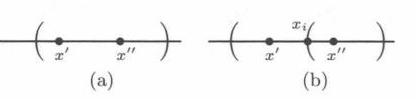
\includegraphics[width=.45\linewidth]{figures/upper/ch03/fig-3-1.png}
\end{center}

(a) 在闭区间 $[x',x'']$ 内没有端点集 $A$ 中的点。于是在 (3.1) 中覆盖该闭区间中任何一点的开区间也就覆盖了整个闭区间。

(b) 在闭区间 $[x',x'']$ 内有 $A$ 中的点。由于数 $\delta$ 的取法，这样的点只有一个。在图 3.1(b) 中将这个点记为 $x_i$，于是有 $x'\leqslant x_i\leqslant x''$。由于这个点 $x_i$ 是 (3.1) 中的开区间的端点，而这个开区间并不覆盖点 $x_i$，因此在 (3.1) 中一定另有开区间覆盖点 $x_i$，它的左右端点必然分别小于 $x'$ 和大于 $x''$，从而也就同时覆盖点 $x'$ 和 $x''$。
\end{xproof}

\begin{xremark}
这个例题是覆盖定理的加强，在今后会看到由于有了这种加强形式，覆盖定理变得更为有力（例如例题 5.2.2，例题 5.4.1 和命题 10.1.5 等）。
\end{xremark}

\subsection{练习题}

\begin{xexercise}[1]
对开区间 $(0,1)$ 构造一个开覆盖，使得它的每一个有限子集都不能覆盖 $(0,1)$。
\end{xexercise}
\begin{xsolution}
取
\[
  O_n=(1/n,1),\qquad n=2,3,\ldots.
\]
任意 $x\in(0,1)$，取 $n>1/x$，则 $1/n<x<1$，故
\[
  (0,1)=\bigcup_{n=2}^{\infty}O_n.
\]
但任取有限多个 $O_{n_1},\ldots,O_{n_k}$，令 $N=\max\{n_1,\ldots,n_k\}$，则
\[
  \bigcup_{j=1}^{k}O_{n_j}=(1/N,1),
\]
它漏掉了 $(0,1/N]$ 中的点。因此没有有限子覆盖。
\end{xsolution}


\begin{xexercise}[2]
用闭区间套定理证明覆盖定理。
\end{xexercise}
\begin{xsolution}
设闭区间 $[a,b]$ 有开覆盖 $\{O_\alpha\}$。反设不存在有限子覆盖。二分 $[a,b]$，若两个半区间都有有限子覆盖，把两组有限子覆盖合并便得到 $[a,b]$ 的有限子覆盖，矛盾。因此至少有一个半区间没有有限子覆盖，把它记为 $I_1$。

继续二分 $I_1$。若它的两个半区间都有有限子覆盖，则合并这两个有限子覆盖就会覆盖 $I_1$，与 $I_1$ 的选取矛盾。因此仍至少有一个半区间没有有限子覆盖，记为 $I_2$。归纳得到闭区间套
\[
  I_1\supset I_2\supset\cdots,
\]
其中每个 $I_n$ 都没有有限子覆盖，而且
\[
  \abs{I_n}=2^{-n}(b-a)\to0.
\]
由闭区间套定理，存在唯一 $\xi\in\bigcap_{n=1}^{\infty}I_n$。

因为 $\{O_\alpha\}$ 覆盖 $[a,b]$，存在某个 $O_{\alpha_0}$ 使 $\xi\in O_{\alpha_0}$。因 $O_{\alpha_0}$ 是开区间，可取 $\delta>0$ 使
\[
  (\xi-\delta,\xi+\delta)\subset O_{\alpha_0}.
\]
取 $n$ 足够大使 $\abs{I_n}<\delta$。由于 $\xi\in I_n$，整个 $I_n$ 都包含在 $(\xi-\delta,\xi+\delta)$ 中，因而单个 $O_{\alpha_0}$ 就覆盖 $I_n$。这与 $I_n$ 没有有限子覆盖矛盾。因此 $[a,b]$ 必有有限子覆盖。
\end{xsolution}


\begin{xexercise}[3]
用覆盖定理证明闭区间套定理。
\end{xexercise}
\begin{xsolution}
设 $I_n=[a_n,b_n]$ 为闭区间套。先证交集非空。反设
\[
  \bigcap_{n=1}^{\infty}I_n=\varnothing.
\]
于是对每个 $x\in I_1$，存在某个 $n$ 使 $x\notin I_n$，即 $x<a_n$ 或 $x>b_n$。因此开区间族
\[
  \{(a_1-1,a_n),(b_n,b_1+1)\mid n\in\NN_+\}
\]
覆盖 $I_1$。由覆盖定理，可取其中有限多个开区间覆盖 $I_1$。设这些开区间所涉及的最大下标为 $N$。由于 $\{a_n\}$ 单调不减而 $\{b_n\}$ 单调不增，这个有限子覆盖的并包含于
\[
  (a_1-1,a_N)\cup(b_N,b_1+1),
\]
但右边漏掉了非空闭区间 $I_N=[a_N,b_N]\subset I_1$，矛盾。因此
\[
  \bigcap_{n=1}^{\infty}I_n\neq\varnothing.
\]

若再有 $\abs{I_n}=b_n-a_n\to0$，而交集中存在两个不同点 $x<y$，则对每个 $n$ 都有 $x,y\in I_n$，从而
\[
  b_n-a_n\geqslant y-x>0,
\]
与 $\abs{I_n}\to0$ 矛盾。故这时交集只能是单点集。
\end{xsolution}


\begin{xexercise}[4]
用覆盖定理证明凝聚定理。
\end{xexercise}
\begin{xsolution}
设有界数列 $\{x_n\}$ 的所有项都在某个闭区间 $[a,b]$ 中。反设它没有收敛子列。于是对每个 $\xi\in[a,b]$，必存在 $\xi$ 的一个开邻域 $O(\xi)$，其中只含数列的有限多项；否则若 $\xi$ 的每个邻域都含无穷多项，就可依次在半径 $1/k$ 的邻域中选取下标递增的 $x_{n_k}$，得到 $x_{n_k}\to\xi$。

于是 $\{O(\xi)\mid\xi\in[a,b]\}$ 是 $[a,b]$ 的开覆盖。由覆盖定理，有有限子覆盖
\[
  O(\xi_1),\ldots,O(\xi_m).
\]
每个邻域中只含原数列的有限多项，因此这有限个邻域的并也只能含有限多项；但它们覆盖 $[a,b]$，而原数列的所有项都在 $[a,b]$ 中，矛盾。故有界数列必有收敛子列。
\end{xsolution}


\begin{xexercise}[5]
试对例题 3.5.2 的证明举出两个具体例子，即 (1) 数集 $A$ 无上界；(2) $A$ 有上界，且有 $b<\xi=\sup A$ 和 $\xi\notin A$。
\end{xexercise}
\begin{xsolution}
在例题 3.5.2 中，固定左端点 $a$，定义
\[
  A=\{x\geqslant a\mid [a,x]\text{ 有有限子覆盖}\}.
\]
可取以下具体例子。
\begin{enumerate}[label=(\arabic*)]
  \item 令 $a=0,b=1$，开覆盖族取
  \[
    O_m=(-1,m),\qquad m\in\NN_+.
  \]
  它当然覆盖 $[0,1]$。对任意 $x\geqslant0$，选整数 $m>x$，则单个 $O_m$ 已覆盖 $[0,x]$，所以
  \[
    A=[0,+\infty),
  \]
  无上界。

  \item 仍令 $a=0,b=1$，只取一个开区间
  \[
    O=(-1,2).
  \]
  它覆盖 $[0,1]$。这时 $[0,x]$ 能被该开覆盖有限覆盖，当且仅当 $0\leqslant x<2$。因此
  \[
    A=[0,2),\qquad \xi=\sup A=2>b=1,
  \]
  且 $2\notin A$。
\end{enumerate}
\end{xsolution}


\section{数列的上极限和下极限}

数列的上、下极限概念是第二章内容的自然延伸。由于其中需要较多的工具，引入的概念和方法也较为精细，因此放在这里讨论。

\subsection{基本定义}

数列的上极限和下极限有几个等价的定义，其中最直观的是用极限点来定义。本书将用极限点来定义上、下极限，其他定义则以命题的形式给出。

\begin{enumerate}
  \item 数列的极限点就是数列的收敛子列的极限。这里约定：

  若存在正（负）无穷大量的子列，则将 $+\infty$（$-\infty$）也作为极限点。因此一个无上界（无下界）数列的极限点中一定有 $+\infty$（$-\infty$）。为区别起见，称收敛子列的极限为有限极限点，而将 $+\infty$ 和 $-\infty$ 称为无限极限点。
  \item 在上述定义下，数列必有极限点（证明见命题 3.6.1）。
  \item 数列的上极限是数列的最大极限点，数列的下极限是数列的最小极限点。这里在比较大小时将 $+\infty,-\infty$ 都作为数来对待。这里最大极限点和最小极限点的存在性也就是上、下极限的存在性，将在命题 3.6.2 中证明。
  \item 从以上定义可以知道，如果存在上极限（下极限），则一定唯一。
  \item 数列 $\{x_n\}$ 的上极限记为 $\overline{\lim}_{n\to\infty}x_n$，下极限记为 $\underline{\lim}_{n\to\infty}x_n$。（在文献中也用记号 $\limsup_{n\to\infty}x_n$ 和 $\liminf_{n\to\infty}x_n$ 来表示数列 $\{x_n\}$ 的上极限和下极限。）
\end{enumerate}

\subsection{基本性质}

首先列出从上、下极限定义即可得到的简单性质：

\begin{enumerate}
  \item 从定义即知
  \[
    \underline{\lim}_{n\to\infty}x_n\leqslant\overline{\lim}_{n\to\infty}x_n.
  \]
  \item 由于数列收敛的充分必要条件是它的每个子列收敛于同一极限，因此即有：数列 $\{x_n\}$ 收敛的充分必要条件是它的上极限和下极限均为有限且相等。
  \item 类似地可以知道，数列为正无穷大量（负无穷大量）的充分必要条件是它的上极限和下极限都是 $+\infty$（$-\infty$）。
  \item 以上两点可以综合为：数列 $\{x_n\}$ 收敛或为有确定符号的无穷大量的充分必要条件是数列的上极限和下极限相等，而且在这时成立
  \[
    \underline{\lim}_{n\to\infty}x_n
    =\overline{\lim}_{n\to\infty}x_n
    =\lim_{n\to\infty}x_n.
  \]
  \item 上、下极限的其他几个简单性质（证明从略）：
  \begin{enumerate}[label=(\arabic*)]
    \item $\overline{\lim}_{n\to\infty}(-x_n)=-\underline{\lim}_{n\to\infty}x_n$；
    \item $\underline{\lim}_{n\to\infty}(-x_n)=-\overline{\lim}_{n\to\infty}x_n$；
    \item 若 $C>0$，则 $\overline{\lim}_{n\to\infty}(Cx_n)=C\overline{\lim}_{n\to\infty}x_n$；
    \item 若 $C<0$，则 $\overline{\lim}_{n\to\infty}(Cx_n)=C\underline{\lim}_{n\to\infty}x_n$。
  \end{enumerate}

  （在这里若出现带确定符号的无穷大量，则按 $-(+\infty)=-\infty$，$-(-\infty)=+\infty$ 等方式来理解。）
\end{enumerate}

下面以命题的形式介绍上、下极限的一些重要性质，其中包括了它们的等价定义，这些定义实际上是从几个不同的角度刻画出上、下极限的特性。

\begin{xproposition}[3.6.1]
证明：任何数列必有极限点。
\end{xproposition}
\begin{xproof}
这里只需要应用例题 3.3.1 的结论，即任何数列都有单调子列。如果这个子列有界，就得到有限极限点；如果它无界，就得到无限极限点。
\end{xproof}

在上一小节给出的上、下极限定义中并未证明最大极限点和最小极限点的存在性，因此这样的定义是不完整的。下一个命题给出上、下极限的第二个等价定义，证明上、下极限的存在性，同时还给出它们的显式表示。

\begin{xproposition}[3.6.2]
每个数列 $\{x_n\}$ 都存在上极限和下极限，且成立公式
\begin{equation}
  \overline{\lim}_{n\to\infty}x_n
  =\lim_{n\to\infty}\sup_{k\geqslant n}\{x_k\},
  \tag{3.2}
  \label{eq:3.2}
\end{equation}
\begin{equation}
  \underline{\lim}_{n\to\infty}x_n
  =\lim_{n\to\infty}\inf_{k\geqslant n}\{x_k\}.
  \tag{3.3}
  \label{eq:3.3}
\end{equation}
\end{xproposition}
\begin{xproof}
在这里只证下极限的存在性和公式 (3.3) 成立。在这以后可以利用
\[
  \overline{\lim}_{n\to\infty}x_n
  =-\underline{\lim}_{n\to\infty}(-x_n)
\]
来证明上极限存在和 (3.2) 成立（这一步请读者完成）。

首先分析公式 (3.3) 的右边。引入记号
\begin{equation}
  b_n=\inf_{k\geqslant n}\{x_k\}
  =\inf\{x_n,x_{n+1},\cdots\},\qquad n\in\NN_+,
  \tag{3.4}
  \label{eq:3.4}
\end{equation}
就可以将 (3.3) 的右边记为 $b=\lim_{n\to\infty}b_n$。

这时要区分两种可能的情况。

(1) 如果有某个 $b_n$ 不是有限数，则从 (3.4) 可见这个 $b_n$ 不可能是 $+\infty$，而只能是 $-\infty$。这时从 (3.4) 可见数列 $\{x_n\}$ 无下界，从而推出每个 $b_n$，$n\in\NN_+$，都是 $-\infty$。这时在等式 (3.3) 的右边只能约定为 $b=\lim_{n\to\infty}b_n=-\infty$。另一方面，由于这时 $\{x_n\}$ 无下界，因此它有一个无限极限点 $-\infty$。这就证明了数列 $\{x_n\}$ 的下极限是 $-\infty$，同时公式 (3.3) 成立。

(2) 在数列 $\{b_n\}$ 的每一项为有限数时，从 (3.4) 可见数列 $\{b_n\}$ 一定是单调增加数列。因此记号 $b=\lim_{n\to\infty}b_n$ 一定有意义。这时又要分两种情况来讨论。

(i) 当 $\{b_n\}$ 无上界时就有 $b=+\infty$。从 (3.4) 可见 $b_n\leqslant x_n$。由于 $\{b_n\}$ 是单调增加的正无穷大量，因此可推出 $\lim_{n\to\infty}x_n=+\infty$。这时数列 $\{x_n\}$ 的唯一极限点是 $+\infty$。因此数列 $\{x_n\}$ 的下极限是 $+\infty$，同时公式 (3.3) 成立。

(ii) 最后一种情况是 $b=\lim_{n\to\infty}b_n$ 为有限数。这时要分两步来做。首先，我们要从数列 $\{x_n\}$ 中寻找一个子列，使它以 $b$ 为极限。这样就可以证明 $b$ 是数列 $\{x_n\}$ 的一个极限点。

对 $\varepsilon=1$，因 $\{b_n\}$ 单调增加收敛于 $b$，就有某个 $b_{k_1}$ 满足 $b-1<b_{k_1}\leqslant b<b+1$。根据 $b_{k_1}=\inf\{x_{k_1},x_{k_1+1},\cdots\}$，存在 $x_{n_1}$（$n_1\geqslant k_1$）满足 $b_{k_1}\leqslant x_{n_1}<b+1$，从而有
\[
  b-1<x_{n_1}<b+1.
\]
同理对 $\varepsilon=\frac12$，有 $k_2>n_1$，使 $b_{k_2}$ 满足 $b-\frac12<b_{k_2}\leqslant b<b+\frac12$。根据 $b_{k_2}=\inf\{x_{k_2},x_{k_2+1},\cdots\}$，存在 $x_{n_2}$（$n_2\geqslant k_2>n_1$）满足 $b_{k_2}\leqslant x_{n_2}<b+\frac12$，从而有
\[
  b-\frac12<x_{n_2}<b+\frac12.
\]
这样归纳地做下去，就可以得到子列 $\{x_{n_k}\}$，对于每个 $k\in\NN_+$，满足
\[
  b-\frac1k<x_{n_k}<b+\frac1k.
\]
既然这个子列以 $b$ 为极限，因此 $b$ 是数列 $\{x_n\}$ 的一个极限点。

第二步是要证明 $b$ 是数列 $\{x_n\}$ 的最小极限点。假设 $c$ 是数列 $\{x_n\}$ 的另一个极限点，则有子列 $\{x_{n'_k}\}$，成立
\[
  \lim_{k\to\infty}x_{n'_k}=c.
\]
在 (3.4) 中令 $n=n'_k$，就有不等式
\[
  b_{n'_k}\leqslant x_{n'_k}.
\]
令 $k\to\infty$，就得到 $b\leqslant c$。这样我们就证明了 $b$ 确实是数列 $\{x_n\}$ 的最小极限点。根据下极限的定义，可见下极限存在，同时成立公式 (3.3)。
\end{xproof}

下面实际上是上极限和下极限的又一个等价定义，它和数列收敛的 $\varepsilon$--$N$ 定义最为接近。为简要起见，只讨论下极限，读者可以对上极限作相应的讨论。

\begin{xproposition}[3.6.3]
(1) 有限数 $b$ 是数列 $\{x_n\}$ 的下极限的充分必要条件是：对每个 $\varepsilon>0$，在邻域 $(b-\varepsilon,b+\varepsilon)$ 中有数列中的无限多项，同时存在 $N$，当 $n>N$ 时，成立不等式 $x_n>b-\varepsilon$；(2) $+\infty$ 是数列 $\{x_n\}$ 的下极限的充分必要条件是 $\{x_n\}$ 为正无穷大量；(3) $-\infty$ 是数列 $\{x_n\}$ 的下极限的充分必要条件是 $\{x_n\}$ 无下界。
\end{xproposition}
\begin{xproof}
(2) 和 (3) 已包含在下极限的定义和上一命题中，因此只须证明 (1)。

先证 (1) 的必要性。因为 $b$ 是数列 $\{x_n\}$ 的有限极限点，因此 $b$ 是某一个子列 $\{x_{n_k}\}$ 的极限，从而对每个 $\varepsilon>0$，在邻域 $(b-\varepsilon,b+\varepsilon)$ 中含有这个子列从某项之后的所有项，当然也就含有数列 $\{x_n\}$ 中的无限多项。又可断言数列 $\{x_n\}$ 中满足条件 $x_n\leqslant b-\varepsilon$ 的项至多只有有限个。否则就可以找出一个子列，使它的每一项都满足这个不等式。用凝聚定理于这个子列，就得到比 $b$ 还要小的极限点，这与 $b$ 是最小极限点相矛盾。因此对 $\varepsilon>0$，有 $N$，当 $n>N$ 时，$x_n>b-\varepsilon$。

再证 (1) 的充分性。令 $\varepsilon=1$，因在 $(b-1,b+1)$ 中有数列 $\{x_n\}$ 中的无限多项，可任取其中一项为 $x_{n_1}$。再令 $\varepsilon=\frac12$，由于在 $(b-\frac12,b+\frac12)$ 中含有数列中的无限多项，因此能取到其中的一项作为 $x_{n_2}$，满足 $n_2>n_1$。归纳地进行下去，就可以得到子列 $\{x_{n_k}\}$，满足要求
\[
  \abs{x_{n_k}-b}<\frac1k,\qquad k\in\NN_+,
\]
因此这个子列收敛于 $b$。这就说明 $b$ 是数列 $\{x_n\}$ 的极限点。

任取一个 $b'<b$，令
\[
  \varepsilon=\frac{b-b'}2,
\]
从条件知有 $N$，当 $n>N$ 时，成立不等式 $x_n>b-\varepsilon=b'+\varepsilon>b'$。因此比 $b$ 小的 $b'$ 不可能是极限点。
\end{xproof}

下一个命题是上、下极限的重要性质，它在应用中往往起关键作用。

\begin{xproposition}[3.6.4]
不等式
\begin{equation}
  \overline{\lim}_{n\to\infty}(x_n+y_n)
  \leqslant\overline{\lim}_{n\to\infty}x_n
  +\overline{\lim}_{n\to\infty}y_n,
  \tag{3.5}
  \label{eq:3.5}
\end{equation}
\begin{equation}
  \underline{\lim}_{n\to\infty}(x_n+y_n)
  \geqslant\underline{\lim}_{n\to\infty}x_n
  +\underline{\lim}_{n\to\infty}y_n
  \tag{3.6}
  \label{eq:3.6}
\end{equation}
在右边有意义（即不是 $+\infty$ 与 $-\infty$ 之和）时成立。
\end{xproposition}
\begin{xproof}
\textbf{证 1}\quad 这里只写出第二个不等式 (3.6) 的证明。证明的方法是用下极限的表达式 (3.3)，先建立不等式
\begin{equation}
  \inf_{k\geqslant n}\{x_k+y_k\}
  \geqslant\inf_{k\geqslant n}\{x_k\}
  +\inf_{k\geqslant n}\{y_k\},
  \tag{3.7}
  \label{eq:3.7}
\end{equation}
然后取极限。如果其中出现的下确界都是有限数，可以记 $A=\inf_{k\geqslant n}\{x_k\}$，$B=\inf_{k\geqslant n}\{y_k\}$。由于对每个 $k\geqslant n$，有 $x_k\geqslant A$ 和 $y_k\geqslant B$，就有 $x_k+y_k\geqslant A+B$。在这里右边是常数，左边对 $k\geqslant n$ 取下确界，就得到所要的不等式 (3.7)。然后在两边令 $n\to\infty$，因为出现在两边的三个数列都是单调增加的，因此不论是收敛还是正无穷大量都是有意义的。这样就得到所求证的公式。

再考虑在不等式 (3.7) 中出现非有限数的情况。根据下确界的定义，在 (3.7) 中只可能出现 $-\infty$。从上一个命题已经知道，下极限为 $-\infty$ 就是数列无下界的情况。这时在命题 3.6.2 中的公式 (3.3) 的右边只是一种约定的记号，并非极限过程。因此不如直接观察所求证的不等式 (3.6)。

分析各种可能性。(1) 若数列 $\{x_n\}$ 和 $\{y_n\}$ 都无下界，则不论不等式 (3.6) 的左边如何，不等式右边的每一项都是 $-\infty$，结论总是成立的。(2) 在两个数列中一个无下界，另一个不是正无穷大量。这时不等式 (3.6) 的右边为 $-\infty$ 与一个有限数之和。只要将这样的和理解为 $-\infty$，则不论不等式左边如何，仍然成立。

\textbf{证 2}\quad 这个证明完全依赖于极限点概念。为简单起见，只对于所出现的极限点均为有限数的情况写出证明。记
\[
  A=\underline{\lim}_{n\to\infty}(x_n+y_n),\qquad
  B=\underline{\lim}_{n\to\infty}x_n,\qquad
  C=\underline{\lim}_{n\to\infty}y_n.
\]
由于 $A$ 是数列 $\{x_n+y_n\}$ 的极限点，因此有子列 $\{x_{n_k}+y_{n_k}\}$ 收敛于 $A$，即
\[
  \lim_{n\to\infty}(x_{n_k}+y_{n_k})=A.
\]
这时可不妨假定 $\{x_{n_k}\}$ 也收敛，否则由于 $\{x_{n_k}\}$ 为有界数列，由凝聚定理知它有收敛子列 $\{x_{n_{k_j}}\}$，于是可以用 $\{x_{n_{k_j}}+y_{n_{k_j}}\}$ 代替 $\{x_{n_k}+y_{n_k}\}$ 作以下讨论。

在 $\{x_{n_k}\}$ 收敛时，$\{y_{n_k}\}$ 也收敛。又因为 $B$ 是 $\{x_n\}$ 的最小极限点，$C$ 是 $\{y_n\}$ 的最小极限点，因此就得到
\[
  \lim_{n\to\infty}x_{n_k}\geqslant B
  \quad\text{和}\quad
  \lim_{n\to\infty}y_{n_k}\geqslant C.
\]
将两式相加就有所要的不等式 $A\geqslant B+C$。
\end{xproof}

\begin{xremark}
由于下极限可以是 $+\infty$ 或 $-\infty$，因此 (3.6) 右边无意义的情况确实可能发生。这就是在数列 $\{x_n\}$ 和 $\{y_n\}$ 中有一个无下界，而另一个为正无穷大量的情况。这时 (3.6) 的左边可以出现各种可能性，但右边无意义，因此 (3.6) 不能成立。
\end{xremark}

下一个命题也是上、下极限的基本性质。它的证明与上一个命题类似，从略。

\begin{xproposition}[3.6.5]
不等式
\[
  \underline{\lim}_{n\to\infty}(x_n+y_n)
  \leqslant\underline{\lim}_{n\to\infty}x_n
  +\overline{\lim}_{n\to\infty}y_n
  \leqslant\overline{\lim}_{n\to\infty}(x_n+y_n)
\]
在中间的和式有意义时成立。
\end{xproposition}

\begin{xremark}
合并以上两个命题就得到以下一组不等式：
\[
  \underline{\lim}_{n\to\infty}x_n+\underline{\lim}_{n\to\infty}y_n
  \leqslant\underline{\lim}_{n\to\infty}(x_n+y_n)
  \leqslant\underline{\lim}_{n\to\infty}x_n+\overline{\lim}_{n\to\infty}y_n
\]
\[
  \leqslant\overline{\lim}_{n\to\infty}(x_n+y_n)
  \leqslant\overline{\lim}_{n\to\infty}x_n+\overline{\lim}_{n\to\infty}y_n,
\]
只要假定其中的和式均有意义。
\end{xremark}

由此又可推出在上、下极限应用中很有用的下列结论。

\begin{xproposition}[3.6.6]
若在数列 $\{x_n\}$ 和 $\{y_n\}$ 中已知 $\{y_n\}$ 收敛，或为带有确定符号的无穷大量时，则成立
\[
  \underline{\lim}_{n\to\infty}(x_n+y_n)
  =\underline{\lim}_{n\to\infty}x_n+\lim_{n\to\infty}y_n,
\]
\[
  \overline{\lim}_{n\to\infty}(x_n+y_n)
  =\overline{\lim}_{n\to\infty}x_n+\lim_{n\to\infty}y_n.
\]
（在 $\{y_n\}$ 为无穷大量时要求所出现的和式有意义。）
\end{xproposition}

\subsection{例题}

\begin{xexample}[3.6.1]
用上、下极限方法证明 Cauchy 收敛准则的充分性部分。
\end{xexample}
\begin{xproof}
\textbf{证 1}\quad 设 $\{x_n\}$ 是基本数列，则 $\forall\varepsilon>0$，$\exists N$，$\forall n>N$，$p\in\NN_+$，成立
\[
  \abs{x_n-x_{n+p}}<\varepsilon.
\]
将这个不等式改写为 $x_n-\varepsilon<x_{n+p}<x_n+\varepsilon$，然后固定某一个 $n$（$>N$），令 $p\to\infty$，由于不论数列收敛与否，总存在上极限和下极限，因而就有
\[
  x_n-\varepsilon\leqslant\underline{\lim}_{n\to\infty}x_n
  \leqslant\overline{\lim}_{n\to\infty}x_n\leqslant x_n+\varepsilon.
\]
上述不等式还表明基本数列的上极限和下极限一定都是有限数（因此基本数列必有界也已得到）。由上述不等式可推出
\[
  0\leqslant\overline{\lim}_{n\to\infty}x_n
  -\underline{\lim}_{n\to\infty}x_n\leqslant2\varepsilon.
\]
由于 $\varepsilon>0$ 可任意给定，可见夹在 $0$ 和 $2\varepsilon$ 中间的两个数只能相等。这样就推出上极限和下极限相等，因此数列 $\{x_n\}$ 收敛。

\textbf{证 2}\quad 设 $\{x_n\}$ 是基本数列。对每个 $\varepsilon>0$，存在 $N$，当 $n,m>N$ 时，成立 $\abs{x_n-x_m}<\varepsilon$。将它改写为 $x_m-\varepsilon<x_n<x_m+\varepsilon$，在后一个不等式中固定 $x_n$，令 $m\to\infty$，利用命题 3.6.6，就得到
\[
  x_n\leqslant\underline{\lim}_{m\to\infty}(x_m+\varepsilon)
  =\underline{\lim}_{m\to\infty}x_m+\varepsilon
  =\underline{\lim}_{n\to\infty}x_n+\varepsilon.
\]
由于这对每个 $n>N$ 成立，而右边是固定数，在左边取上极限，就得到
\[
  \overline{\lim}_{n\to\infty}x_n
  \leqslant\underline{\lim}_{n\to\infty}x_n+\varepsilon.
\]
以上推导还表明 $\{x_n\}$ 的上、下极限都是有限数。最后，利用 $\varepsilon$ 的任意性，就有
\[
  \overline{\lim}_{n\to\infty}x_n
  \leqslant\underline{\lim}_{n\to\infty}x_n.
\]
由于相反方向的不等式总是成立的，因此成立
\[
  \overline{\lim}_{n\to\infty}x_n
  =\underline{\lim}_{n\to\infty}x_n,
\]
即数列 $\{x_n\}$ 收敛。
\end{xproof}

\begin{xremark}
教科书 [33] 在数列极限一章中就讲授上、下极限，并用于证明 Cauchy 收敛准则。其中所用的就是上述第一个证明。
\end{xremark}

再给出上、下极限在迭代生成数列问题中的一个应用（参见例题 3.4.5），其中用到的有关上、下极限的知识请读者自己证明。

\begin{xexample}[3.6.2]
设数列 $\{b_n\}$ 由 $b_1=1$ 和 $b_{n+1}=1+\frac1{b_n}$ 生成。讨论数列 $\{b_n\}$ 的敛散性，若收敛则求出其极限。
\end{xexample}
\begin{xsolution}
设已证明数列 $\{b_n\}$ 从第二项起不越出区间 $[1.5,2]$，因此有
\[
  1.5\leqslant\alpha=\underline{\lim}_{n\to\infty}b_n
  \leqslant\beta=\overline{\lim}_{n\to\infty}b_n\leqslant2.
\]
在递推公式两边取上极限和下极限，得到
\[
  \alpha=1+\underline{\lim}_{n\to\infty}\left(\frac1{b_n}\right)
  =1+\frac1{\overline{\lim}_{n\to\infty}b_n}
  =1+\frac1\beta
\]
和对称的
\[
  \beta=1+\overline{\lim}_{n\to\infty}\left(\frac1{b_n}\right)
  =1+\frac1{\underline{\lim}_{n\to\infty}b_n}
  =1+\frac1\alpha.
\]
将这两个方程联立，相减后得到
\[
  (\alpha-\beta)\left(1-\frac1{\alpha\beta}\right)=0.
\]
由于 $\beta\geqslant\alpha\geqslant1.5$，即可得到 $\alpha=\beta$，即数列收敛。然后再求出极限（从略）。
\end{xsolution}

以下是用上、下极限方法于第二章第二组参考题 14。

\begin{xexample}[3.6.3]
设 $y_n=x_n+2x_{n+1}$，$n\in\NN_+$。证明：若 $\{y_n\}$ 收敛，则 $\{x_n\}$ 也收敛。
\end{xexample}
\begin{xproof}
由于 $\{y_n\}$ 收敛，因此它有界。取正数 $M>0$ 使同时成立 $\abs{x_1}\leqslant M$ 和 $\abs{y_n}\leqslant M$，$n\in\NN_+$。将递推公式改写为 $x_{n+1}=\frac12y_n-\frac12x_n$，则有
\[
  \abs{x_{n+1}}\leqslant\frac12\abs{y_n}+\frac12\abs{x_n}.
\]
因此，用数学归纳法可以知道 $\abs{x_n}\leqslant M$ 对每个 $n$ 成立，即数列 $\{x_n\}$ 有界。

记
\[
  \overline{\lim}_{n\to\infty}x_n=A,\qquad
  \underline{\lim}_{n\to\infty}x_n=B
  \quad\text{和}\quad
  \lim_{n\to\infty}y_n=C,
\]
则它们都是有限数。只要证明 $A=B$。在 $x_n=y_n-2x_{n+1}$ 两边分别取上极限和下极限，由于 $\{y_n\}$ 收敛，可以利用命题 3.6.6，得到等式 $A=C-2B$ 和 $B=C-2A$，由此推出 $A=B$。
\end{xproof}

\begin{xremark}
有了上、下极限的新工具，不必知道数列收敛就可以进行上、下极限运算。请读者将这个方法与过去的方法对比，并在其他问题上尝试一下。在第二章中的不少问题都有可能用上、下极限的新工具来做，以上的两个例题仅供参考。
\end{xremark}

下一个例题与确界和上、下极限都有关系。它（以及它的变形）出现在多个领域的研究中，可以说是上、下极限的一个重要应用。

\begin{xexample}[3.6.4]
设正数列 $\{a_n\}$ 满足条件
\[
  a_{n+m}\leqslant a_na_m,\qquad \forall n,m\in\NN_+,
\]
则有
\[
  \lim_{n\to\infty}\frac{\ln a_n}{n}
  =\inf_{n\geqslant1}\left\{\frac{\ln a_n}{n}\right\}.
\]
\end{xexample}
\begin{xproof}
令
\[
  \alpha=\inf_{n\geqslant1}\left\{\frac{\ln a_n}{n}\right\},
\]
则从命题 (3.6.2) 的公式 (3.3) 可见有
\begin{equation}
  \alpha\leqslant\underline{\lim}_{n\to\infty}\frac{\ln a_n}{n}.
  \tag{3.8}
  \label{eq:3.8}
\end{equation}
又从 $\alpha$ 为下确界（即最大下界）可见，对 $\varepsilon>0$，存在 $N$，使得
\[
  \frac{\ln a_N}{N}<\alpha+\varepsilon.
\]
固定这个 $N$，可以将每个正整数 $n$ 写为 $n=mN+k$，其中 $0\leqslant k<N$。从题设条件，有不等式
\[
  a_n=a_{mN+k}\leqslant a_N^ma_k,
\]
取对数后可以得到
\[
  \frac{\ln a_n}{n}
  \leqslant\frac{m}{n}\ln a_N+\frac1n\ln a_k
  <\frac{mN}{n}(\alpha+\varepsilon)+\frac1n\ln a_k.
\]
在这个不等式两边令 $n\to\infty$，右边第一项中有极限
\[
  \lim_{n\to\infty}\frac{mN}{n}=1,
\]
而 $a_k$ 最多只取 $N$ 个值，因此右边的极限是 $\alpha+\varepsilon$。左边的极限虽然不知道是否存在，但可利用上极限的保不等式性质（作为练习题），在不等式两边取上极限，从而得到
\[
  \overline{\lim}_{n\to\infty}\frac{\ln a_n}{n}\leqslant\alpha+\varepsilon.
\]
由于 $\varepsilon>0$ 的任意性，就得到
\[
  \overline{\lim}_{n\to\infty}\frac{\ln a_n}{n}\leqslant\alpha.
\]
将这个不等式与 (3.8) 合并，可见 $\lim_{n\to\infty}\frac{\ln a_n}{n}$ 一定有意义，且等于 $\alpha$。
\end{xproof}

\begin{xremark}
\textbf{注 1}\quad 上述结论的意思是：当 $\alpha$ 为有限数时数列 $\{\frac{\ln a_n}{n}\}$ 一定收敛，以 $\alpha$ 为极限，而当 $\alpha=-\infty$ 时，这个数列一定是负无穷大量。

\textbf{注 2}\quad 又由此可见，在正数列满足条件 $a_{n+m}\leqslant a_na_m$，$\forall n,m\in\NN_+$ 时，极限
\[
  \lim_{n\to\infty}\sqrt[n]{a_n}
\]
一定存在。

\textbf{注 3}\quad 与此等价的命题是：设 $\{a_n\}$ 满足条件 $a_{n+m}\leqslant a_n+a_m$，$\forall n,m\in\NN_+$，则有
\[
  \lim_{n\to\infty}\frac{a_n}{n}
  =\inf_{n\geqslant1}\left\{\frac{a_n}{n}\right\}.
\]
\end{xremark}

\subsection{练习题}

\begin{xexercise}[1]
求下列数列的上极限和下极限：
  \begin{enumerate}[label=(\arabic*)]
    \item $x_n=\frac{1+(-1)^n}{2}$，$n\in\NN_+$；
    \item $x_n=\sin\frac{n\pi}{4}$，$n\in\NN_+$；
    \item $x_n=n^{(-1)^n}$，$n\in\NN_+$；
    \item $x_n=\ee^{n(-1)^n}$，$n\in\NN_+$。
  \end{enumerate}
\end{xexercise}
\begin{xsolution}
\begin{enumerate}[label=(\arabic*)]
  \item $x_n=(1+(-1)^n)/2$ 的奇数项恒为 $0$、偶数项恒为 $1$，故
  \[
    \underline{\lim}_{n\to\infty}x_n=0,
    \qquad
    \overline{\lim}_{n\to\infty}x_n=1.
  \]

  \item $x_n=\sin(n\pi/4)$ 以周期 $8$ 重复取值
  \[
    \frac{\sqrt2}{2},\ 1,\ \frac{\sqrt2}{2},\ 0,
    -\frac{\sqrt2}{2},\ -1,\ -\frac{\sqrt2}{2},\ 0.
  \]
  因此
  \[
    \underline{\lim}_{n\to\infty}x_n=-1,
    \qquad
    \overline{\lim}_{n\to\infty}x_n=1.
  \]

  \item 对 $x_n=n^{(-1)^n}$，偶数项 $x_{2k}=2k\to+\infty$，奇数项 $x_{2k-1}=1/(2k-1)\to0$。故
  \[
    \underline{\lim}_{n\to\infty}x_n=0,
    \qquad
    \overline{\lim}_{n\to\infty}x_n=+\infty.
  \]

  \item 对 $x_n=\ee^{n(-1)^n}$，偶数项趋于 $+\infty$，奇数项 $\ee^{-n}\to0$。故
  \[
    \underline{\lim}_{n\to\infty}x_n=0,
    \qquad
    \overline{\lim}_{n\to\infty}x_n=+\infty.
  \]
\end{enumerate}
\end{xsolution}


\begin{xexercise}[2]
若 $x_n\geqslant y_n$，$n\in\NN_+$，证明：
  \[
    \overline{\lim}_{n\to\infty}x_n\geqslant\overline{\lim}_{n\to\infty}y_n,
    \qquad
    \underline{\lim}_{n\to\infty}x_n\geqslant\underline{\lim}_{n\to\infty}y_n.
  \]
\end{xexercise}
\begin{xsolution}
对每个 $n$，由 $x_k\geqslant y_k$（$k\geqslant n$）有
\[
  \sup_{k\geqslant n}x_k\geqslant\sup_{k\geqslant n}y_k,
  \qquad
  \inf_{k\geqslant n}x_k\geqslant\inf_{k\geqslant n}y_k.
\]
令 $n\to\infty$，利用上下极限的尾集表示，得到
\[
  \overline{\lim}_{n\to\infty}x_n
  \geqslant\overline{\lim}_{n\to\infty}y_n,
  \qquad
  \underline{\lim}_{n\to\infty}x_n
  \geqslant\underline{\lim}_{n\to\infty}y_n.
\]
\end{xsolution}


\begin{xexercise}[3]
对 $\{x_n\}$，记 $S_n=\frac1n\sum_{k=1}^{n}x_k$，$n\in\NN_+$，证明：
  \[
    \underline{\lim}_{n\to\infty}x_n
    \leqslant\underline{\lim}_{n\to\infty}S_n
    \leqslant\overline{\lim}_{n\to\infty}S_n
    \leqslant\overline{\lim}_{n\to\infty}x_n.
  \]
  （可以看出本题的结论蕴涵了 §2.4 中的 Cauchy 命题。）
\end{xexercise}
\begin{xsolution}
记
\[
  l=\underline{\lim}_{n\to\infty}x_n,
  \qquad
  L=\overline{\lim}_{n\to\infty}x_n.
\]
先设 $l,L$ 都是有限数。任取 $\varepsilon>0$，存在 $N$，当 $k\geqslant N$ 时
\[
  l-\varepsilon<x_k<L+\varepsilon.
\]
于是对 $n\geqslant N$，
\[
  \frac1n\sum_{k=1}^{N-1}x_k
  +\frac{n-N+1}{n}(l-\varepsilon)
  <S_n
\]
以及
\[
  S_n<
  \frac1n\sum_{k=1}^{N-1}x_k
  +\frac{n-N+1}{n}(L+\varepsilon).
\]
令 $n\to\infty$，有限个初始项除以 $n$ 后趋于 $0$，得到
\[
  l-\varepsilon\leqslant\underline{\lim}S_n
  \leqslant\overline{\lim}S_n\leqslant L+\varepsilon.
\]
再令 $\varepsilon\downarrow0$，即得结论。

若 $l$ 有限而 $L=+\infty$，上面的左侧估计仍给出
\[
  l\leqslant\underline{\lim}S_n,
\]
而最右侧不等式自动成立；若 $l=-\infty$ 而 $L$ 有限，则使用上面的右侧估计即可。若 $l=-\infty,L=+\infty$，两个外侧不等式都自动成立。

还剩两种同号无穷情形。若 $l=+\infty$，则对任意实数 $M$，存在 $N$，使 $k\geqslant N$ 时 $x_k>M$。因此
\[
  S_n>
  \frac1n\sum_{k=1}^{N-1}x_k+\frac{n-N+1}{n}M,
  \qquad n\geqslant N.
\]
令 $n\to\infty$ 得 $\underline{\lim}S_n\geqslant M$。因 $M$ 任意，$S_n\to+\infty$。若 $L=-\infty$，对任意实数 $M$ 最终有 $x_k<M$，同样得到 $\overline{\lim}S_n\leqslant M$，故 $S_n\to-\infty$。于是所有扩展实数情形均成立。
\end{xsolution}


\begin{xexercise}[4]
设 $\{a_n\}$ 为正数列，证明：
  \[
    \overline{\lim}_{n\to\infty}\sqrt[n]{a_n}\leqslant1
  \]
  的充分必要条件是对大于 $1$ 的每个数 $l$ 成立
  \[
    \lim_{n\to\infty}\frac{a_n}{l^n}=0.
  \]
\end{xexercise}
\begin{xsolution}
先设
\[
  \overline{\lim}_{n\to\infty}\sqrt[n]{a_n}\leqslant1.
\]
任取 $l>1$，再取 $r$ 满足 $1<r<l$。由上极限定义，存在 $N$，当 $n>N$ 时
\[
  \sqrt[n]{a_n}<r.
\]
于是
\[
  0<\frac{a_n}{l^n}<\left(\frac rl\right)^n\to0,
\]
故 $a_n/l^n\to0$。

反之，假设对每个 $l>1$ 都有 $a_n/l^n\to0$。若
\[
  \overline{\lim}_{n\to\infty}\sqrt[n]{a_n}>1,
\]
则可取 $1<l<r<\overline{\lim}\sqrt[n]{a_n}$。由上极限的定义，有无穷多个 $n$ 满足 $\sqrt[n]{a_n}>r$，从而这些 $n$ 上
\[
  \frac{a_n}{l^n}>\left(\frac rl\right)^n.
\]
右端沿该子列趋于 $+\infty$，与 $a_n/l^n\to0$ 矛盾。因此上极限不超过 $1$。
\end{xsolution}


\begin{xexercise}[5]
设 $\{a_n\}$ 为正数列，证明：
  \[
    \underline{\lim}_{n\to\infty}\frac{a_{n+1}}{a_n}
    \leqslant\underline{\lim}_{n\to\infty}\sqrt[n]{a_n}
    \leqslant\overline{\lim}_{n\to\infty}\sqrt[n]{a_n}
    \leqslant\overline{\lim}_{n\to\infty}\frac{a_{n+1}}{a_n}.
  \]
\end{xexercise}
\begin{xsolution}
记
\[
  r=\underline{\lim}_{n\to\infty}\frac{a_{n+1}}{a_n},
  \qquad
  R=\overline{\lim}_{n\to\infty}\frac{a_{n+1}}{a_n}.
\]
先证右端不等式。若 $R<+\infty$，任取正数 $q>R$。存在 $N$，当 $n\geqslant N$ 时
\[
  \frac{a_{n+1}}{a_n}<q.
\]
故对 $n>N$，
\[
  a_n<a_Nq^{n-N}.
\]
开 $n$ 次方得
\[
  \sqrt[n]{a_n}<a_N^{1/n}q^{1-N/n}.
\]
令 $n\to\infty$，得到
\[
  \overline{\lim}_{n\to\infty}\sqrt[n]{a_n}\leqslant q.
\]
再令 $q\downarrow R$，便有
\[
  \overline{\lim}_{n\to\infty}\sqrt[n]{a_n}\leqslant R.
\]
若 $R=+\infty$，这一不等式自动成立。

再证左端不等式。若 $0<r<+\infty$，任取 $0<q<r$。充分大的 $n$ 有
\[
  \frac{a_{n+1}}{a_n}>q,
\]
从而 $a_n>a_Nq^{n-N}$，于是
\[
  \underline{\lim}_{n\to\infty}\sqrt[n]{a_n}\geqslant q.
\]
令 $q\uparrow r$ 得
\[
  r\leqslant\underline{\lim}_{n\to\infty}\sqrt[n]{a_n}.
\]
若 $r=0$，因 $\sqrt[n]{a_n}>0$，该不等式自动成立；若 $r=+\infty$，上述估计对任意有限 $q>0$ 都成立，故
\[
  \underline{\lim}_{n\to\infty}\sqrt[n]{a_n}=+\infty.
\]
最后
\[
  \underline{\lim}_{n\to\infty}\sqrt[n]{a_n}
  \leqslant
  \overline{\lim}_{n\to\infty}\sqrt[n]{a_n}
\]
由定义成立。合并即得原题的全部不等式。
\end{xsolution}


\begin{xexercise}[6]
根据极限点的定义直接证明：每个数列的极限点集中必有最大数和最小数（不要利用命题 3.6.2 和 3.6.3 的现成结论）。
\end{xexercise}
\begin{xsolution}
先证最大极限点存在，不使用命题 3.6.2、3.6.3。

若 $\{x_n\}$ 无上界，则可递归选取 $n_k$ 使 $x_{n_k}>k$，所以 $x_{n_k}\to+\infty$；按本章约定 $+\infty$ 是极限点，并且在扩展实数的次序中没有比它更大的点，因此它是最大极限点。以下设 $\{x_n\}$ 有上界。

设有限极限点集合为 $E$。若 $E\neq\varnothing$，则 $E$ 有上界。令 $L=\sup E$。对每个 $k$，可取 $c_k\in E$ 使
\[
  L-\frac1k<c_k\leqslant L.
\]
由于 $c_k$ 是极限点，在 $(c_k-1/k,c_k+1/k)$ 中有原数列的无穷多项。于是可递归选取 $n_k>n_{k-1}$ 使
\[
  \abs{x_{n_k}-c_k}<\frac1k.
\]
因此
\[
  \abs{x_{n_k}-L}
  \leqslant\abs{x_{n_k}-c_k}+\abs{c_k-L}<\frac2k,
\]
故 $x_{n_k}\to L$。所以 $L\in E$，即 $L$ 是最大有限极限点。

若 $E=\varnothing$，则数列必须是负无穷大量。否则存在实数 $M$，使得有无穷多项满足 $x_n\geqslant M$；结合数列有上界，这些项组成有界子列，由凝聚定理应有有限极限点，与 $E=\varnothing$ 矛盾。因此此时唯一的极限点是 $-\infty$，它同时也是最大极限点。

最小极限点的存在性完全对称：若数列无下界，则 $-\infty$ 为最小极限点；若有下界且有限极限点非空，对其取下确界并作同样的对角选取；若没有有限极限点，则数列为正无穷大量，唯一极限点为 $+\infty$。故最大、最小极限点都存在。
\end{xsolution}


\begin{xexercise}[7]
证明在例题 3.6.2 中所用到的关于上、下极限的公式。
\end{xexercise}
\begin{xsolution}
例题中 $b_n\in[1.5,2]$，故所有量均为正且有限。记
\[
  \alpha=\underline{\lim}_{n\to\infty}b_n,
  \qquad
  \beta=\overline{\lim}_{n\to\infty}b_n.
\]
删除有限个初始项不改变上下极限，因此
\[
  \underline{\lim}b_{n+1}=\alpha,
  \qquad
  \overline{\lim}b_{n+1}=\beta.
\]
对尾集利用倒数函数在正数上的反序性，有
\[
  \sup_{k\geqslant n}\frac1{b_k}
  =\frac1{\inf_{k\geqslant n}b_k},
  \qquad
  \inf_{k\geqslant n}\frac1{b_k}
  =\frac1{\sup_{k\geqslant n}b_k}.
\]
令 $n\to\infty$，得到
\[
  \overline{\lim}_{n\to\infty}\frac1{b_n}=\frac1\alpha,
  \qquad
  \underline{\lim}_{n\to\infty}\frac1{b_n}=\frac1\beta.
\]
又常数相加可直接移出上下极限。于是由
\[
  b_{n+1}=1+\frac1{b_n}
\]
两边取下极限和上极限，分别得到
\[
  \alpha=1+\frac1\beta,
  \qquad
  \beta=1+\frac1\alpha,
\]
这正是例题中使用的公式。
\end{xsolution}


\begin{xexercise}[8]
证明公式 (3.2)。
\end{xexercise}
\begin{xsolution}
对数列 $\{-x_n\}$ 应用已经证明的公式 (3.3)，有
\[
  \underline{\lim}_{n\to\infty}(-x_n)
  =\lim_{n\to\infty}\inf_{k\geqslant n}(-x_k).
\]
利用
\[
  \overline{\lim}x_n=-\underline{\lim}(-x_n),
  \qquad
  \inf_{k\geqslant n}(-x_k)
  =-\sup_{k\geqslant n}x_k,
\]
两边同乘 $-1$，即得
\[
  \overline{\lim}_{n\to\infty}x_n
  =\lim_{n\to\infty}\sup_{k\geqslant n}x_k.
\]
扩展实数 $\pm\infty$ 的情形也由同一恒等式成立。
\end{xsolution}


\begin{xexercise}[9]
对上极限写出与命题 3.6.3 对应的结论，并作出证明。
\end{xexercise}
\begin{xsolution}
对应结论如下。

(1) 有限数 $b$ 是 $\{x_n\}$ 的上极限，当且仅当对每个 $\varepsilon>0$，邻域 $(b-\varepsilon,b+\varepsilon)$ 中有数列的无穷多项，并且存在 $N$，当 $n>N$ 时
\[
  x_n<b+\varepsilon.
\]

(2) $+\infty$ 是上极限，当且仅当 $\{x_n\}$ 无上界。

(3) $-\infty$ 是上极限，当且仅当 $\{x_n\}$ 为负无穷大量。

证明有限情形。若 $b$ 是上极限，则它是极限点，所以每个邻域有无穷多项。若对某个 $\varepsilon>0$ 有无穷多项满足 $x_n\geqslant b+\varepsilon$，从这些项中取子列；若该子列有界，凝聚定理给出一个不小于 $b+\varepsilon$ 的有限极限点；若无界，则有 $+\infty$ 极限点。两者都与 $b$ 为最大极限点矛盾。因此最终必有 $x_n<b+\varepsilon$。

反之，假设上述两条件成立。由每个邻域中有无穷多项，可递归选取 $n_k$ 使
\[
  \abs{x_{n_k}-b}<\frac1k,
\]
故 $b$ 是极限点。任取 $b'>b$，令 $\varepsilon=(b'-b)/2$。最终有
\[
  x_n<b+\varepsilon=b'-\varepsilon<b',
\]
所以不可能有子列收敛到 $b'$，也不可能有趋于 $+\infty$ 的子列。因此不存在大于 $b$ 的极限点，$b$ 即最大极限点。

无穷情形 (2)、(3) 可由极限点定义直接得到，或对命题 3.6.3 应用于 $-x_n$ 得到。
\end{xsolution}


\begin{xexercise}[10]
证明公式 (3.5)。
\end{xexercise}
\begin{xsolution}
记
\[
  A=\overline{\lim}_{n\to\infty}x_n,
  \qquad
  B=\overline{\lim}_{n\to\infty}y_n,
\]
并假设 $A+B$ 有意义。

先设 $A,B$ 都有限。对充分大的 $n$，记
\[
  A_n=\sup_{k\geqslant n}x_k,
  \qquad
  B_n=\sup_{k\geqslant n}y_k.
\]
对所有 $k\geqslant n$ 有
\[
  x_k+y_k\leqslant A_n+B_n,
\]
所以
\[
  \sup_{k\geqslant n}(x_k+y_k)\leqslant A_n+B_n.
\]
令 $n\to\infty$，由公式 (3.2) 得
\[
  \overline{\lim}_{n\to\infty}(x_n+y_n)
  \leqslant A+B.
\]

若 $A+B=+\infty$，所求不等式自动成立。若 $A+B=-\infty$，由于和式有意义，至少有一个上极限等于 $-\infty$，另一个不为 $+\infty$。例如设 $A=-\infty$。若 $B$ 有限，则任取实数 $M$，最终有
\[
  y_n<B+1,
  \qquad
  x_n<M-(B+1),
\]
因而最终 $x_n+y_n<M$。若 $B=-\infty$，则 $x_n\to-\infty$、$y_n\to-\infty$，同样有 $x_n+y_n\to-\infty$。因此在两种情形中都有
\[
  \overline{\lim}_{n\to\infty}(x_n+y_n)=-\infty=A+B.
\]
若由 $B=-\infty$ 而 $A$ 有限，则交换 $x_n,y_n$ 的地位即可。故所有使右端有意义的扩展实数情形也都成立。
\end{xsolution}


\begin{xexercise}[11]
证明命题 3.6.5。
\end{xexercise}
\begin{xsolution}
记
\[
  a=\underline{\lim}_{n\to\infty}x_n,
  \qquad
  B=\overline{\lim}_{n\to\infty}y_n,
  \qquad
  z_n=x_n+y_n,
\]
并假设 $a+B$ 有意义。需证
\[
  \underline{\lim}z_n\leqslant a+B\leqslant\overline{\lim}z_n.
\]

先设 $a,B$ 都有限。对充分大的 $n$，记
\[
  \alpha_n=\inf_{k\geqslant n}x_k,
  \qquad
  B_n=\sup_{k\geqslant n}y_k.
\]
任取 $\varepsilon>0$。由下确界定义，可取 $k\geqslant n$ 使 $x_k<\alpha_n+\varepsilon$；又 $y_k\leqslant B_n$，所以
\[
  \inf_{j\geqslant n}z_j
  \leqslant z_k<\alpha_n+B_n+\varepsilon.
\]
令 $\varepsilon\downarrow0$，得到
\[
  \inf_{j\geqslant n}z_j\leqslant\alpha_n+B_n.
\]
同样，由上确界定义可取 $k\geqslant n$ 使 $y_k>B_n-\varepsilon$；又 $x_k\geqslant\alpha_n$，故
\[
  \sup_{j\geqslant n}z_j
  \geqslant z_k>\alpha_n+B_n-\varepsilon.
\]
令 $\varepsilon\downarrow0$，得
\[
  \alpha_n+B_n\leqslant\sup_{j\geqslant n}z_j.
\]
再令 $n\to\infty$，即得所需两式。

若 $a+B=+\infty$，左侧不等式自动成立，只需说明 $\overline{\lim}z_n=+\infty$。若 $B=+\infty$ 且 $a>-\infty$，则 $x_n$ 最终有一个有限下界，而 $y_n$ 有趋于 $+\infty$ 的子列，所以相应的 $z_n$ 子列趋于 $+\infty$。剩下的有意义情形是 $a=+\infty$ 而 $B$ 为有限数。由 $B$ 是 $y_n$ 的上极限，可选子列 $y_{n_k}\to B$；同时 $x_{n_k}\to+\infty$，故 $z_{n_k}\to+\infty$。

若 $a+B=-\infty$，右侧不等式自动成立，只需说明 $\underline{\lim}z_n=-\infty$。若 $a=-\infty$ 且 $B<+\infty$，取子列 $x_{n_k}\to-\infty$，而 $y_n$ 最终有有限上界，于是 $z_{n_k}\to-\infty$。剩下的有意义情形是 $B=-\infty$ 而 $a$ 为有限数。可取子列 $x_{n_k}\to a$；同时 $y_{n_k}\to-\infty$，仍有 $z_{n_k}\to-\infty$。因此命题 3.6.5 在所有中间和式有意义的情形下成立。
\end{xsolution}


\section{对于教学的建议}

\subsection{学习要点}

\begin{enumerate}
  \item 本章中相当多的内容都是为数学分析的整个理论展开做准备工作的。对初次接触实数系基本定理的读者来说，应当脚踏实地将每一个定理的条件、结论搞清楚，并至少对每个定理能独立用于证明一个常见的命题或习题。与其他内容的学习一样，看别人的十个现成的题解还不如自己动手做一个题。当然，一开始时不看书上的题解而能将它正确地复述出来也是学习的一种方法。但在这个基础上还是需要自己动手做题。

  \item 另一种方法也可以用，这就是先重点学会其中的一个定理，例如闭区间套定理，由于有 Bolzano 的二分法等方法可用，下手比较容易。初学者可以尝试用它去解决几个问题，如在后面连续函数理论中的许多命题，或用于证明其他基本定理等。在比较熟悉之后再换一个工具。这样分段学习往往比较切合实际，有些教材就是如此进行安排的。

  \item 本章的另一个内容是上、下极限。由于这是数列极限理论中最为精细的部分，又有三个等价定义从不同角度进行刻画，因此对初学者是比较困难的。这方面较难的题很多，除了特别有价值的例题 3.6.4 外，本书均未收入。读者如在这方面有进一步的需要，可以从 [8,44,56] 中找到更多的材料。应当指出，没有上、下极限的极限理论是不完整的。从例题 3.6.1、3.6.2 和 3.6.3 可见上、下极限为很多问题提供了全新的方法，很有价值。

  \item \textbf{对习题课的建议}\quad 如前所述，在整个数学分析的内容中，本章是理论性最强的一章，因此对于初学者来说会有很大的困难。如何进行有良好效果的教学乃是教师和学生共同面临的问题。容易理解，教学中的系统性和可接受性有时难以两全。因此，除了少数教材外（例如 [14,73] 等），在大多数教材中都采取了分散难点的安排方法。本书将它们集中在一章里，便于参考，但应当按照初学者接受知识的规律来使用这些材料。
\end{enumerate}

\subsection{一题多解}

在本节中举一个非常简单的例题，但尝试用每一个基本定理对它作出证明（其中的方法均已出现过），供读者比较。

\begin{xexample}[3.7.1]
如函数 $f$ 在闭区间 $[a,b]$ 上处处局部有界（它的确切含义在证 1 中写出），则函数 $f$ 在 $[a,b]$ 上有界。
\end{xexample}
\begin{xproof}
\textbf{证 1（用覆盖定理为工具）}\quad 函数 $f$ 在 $[a,b]$ 上处处局部有界是指：对每个 $x\in[a,b]$，存在邻域 $O(x)$ 和常数 $M_x$，使得
\[
  \abs{f(x)}<M_x,\qquad \forall x\in O(x)\cap[a,b].
\]
对每个 $x\in[a,b]$ 取定一个 $O(x)$ 和相应的常数 $M_x$，就得到了闭区间 $[a,b]$ 的一个开覆盖。用覆盖定理，在上述开覆盖中存在有限子覆盖，不妨记为 $O_1,O_2,\cdots,O_n$，与它们相应的常数记为 $M_1,M_2,\cdots,M_n$。取 $M=\max\{M_1,M_2,\cdots,M_n\}$，由于
\[
  [a,b]\subset\bigcup_{i=1}^{n}O_i,
\]
可见对于每个 $x\in[a,b]$ 都成立 $\abs{f(x)}<M$，即函数 $f$ 在 $[a,b]$ 上有界。

\textbf{证 2（用闭区间套定理和 Bolzano 二分法为工具）}\quad 用反证法。设 $f$ 在 $[a,b]$ 上无界。记 $a_1=a,b_1=b$。在 $[a_1,b_1]$ 中取中点 $c_1=(a_1+b_1)/2$，得到两个子区间 $[a_1,c_1]$ 和 $[c_1,b_1]$。函数 $f$ 至少在这两个子区间中的某一个上无界，将它取为 $[a_2,b_2]$（若两个子区间上 $f$ 均无界则任取其一）。这是构造的第一步。

继续这样做下去，归纳地得到一个闭区间套 $\{[a_n,b_n]\}$，它具有两个特性：(1) 区间长度所成的数列收敛于 $0$；(2) 每个区间 $[a_n,b_n]$ 上 $f$ 都是无界的。

用闭区间套定理于上述 $\{[a_n,b_n]\}$，知有 $\xi\in[a,b]$，成立
\[
  \lim_{n\to\infty}a_n=\lim_{n\to\infty}b_n=\xi.
\]
由于 $f$ 在 $[a,b]$ 上的局部有界性，对 $\xi$ 存在邻域 $O(\xi)$，使 $f$ 在 $O(\xi)\cap[a,b]$ 上有界。将这个邻域的半径记为 $\varepsilon$，就可以写出 $O(\xi)=(\xi-\varepsilon,\xi+\varepsilon)$。但由于 $\xi$ 是闭区间套的端点所成数列的极限，存在 $N$，使得 $[a_N,b_N]\subset(\xi-\varepsilon,\xi+\varepsilon)$。由于 $f$ 在 $[a_N,b_N]$ 上无界，引出矛盾。

\textbf{证 3（用 Cauchy 收敛准则为工具）}\quad 这个方法的第一步与用闭区间套定理的证明相同。用反证法，构造 $\{[a_n,b_n]\}$，因为 $f$ 在每个 $[a_n,b_n]$ 上无界，存在 $x_n\in[a_n,b_n]$，使得 $\abs{f(x_n)}>n$。由于 $x_n$ 和 $x_{n+p}$（$p\in\NN_+$）都属于 $[a_n,b_n]$，因此有估计
\[
  \abs{x_n-x_{n+p}}<\frac1{2^{n-1}}(b-a).
\]
这表明 $\{x_n\}$ 是基本数列。由 Cauchy 收敛准则知 $\{x_n\}$ 收敛，记其极限为 $\xi$。

由于 $f$ 的局部有界性，存在 $\varepsilon>0$ 和 $M>0$，当 $x\in(\xi-\varepsilon,\xi+\varepsilon)\cap[a,b]$ 时成立 $\abs{f(x)}<M$。又因 $\{x_n\}$ 收敛于 $\xi$，对上述 $\varepsilon>0$，有 $N$，当 $n>N$ 时，成立 $\abs{x_n-\xi}<\varepsilon$。

于是当 $n>N$ 时有 $\abs{f(x_n)}<M$，又对每个 $n$ 有 $\abs{f(x_n)}>n$，引出矛盾。

\textbf{证 4（用单调有界数列的收敛定理为工具）}\quad 用反证法。设 $f$ 在 $[a,b]$ 上无界，则对每个 $n$，存在 $x_n\in[a,b]$，使 $\abs{f(x_n)}>n$。这样得到一个有界数列 $\{x_n\}$。利用例题 3.3.1，在 $\{x_n\}$ 中有单调子列 $\{x_{n_k}\}$ 收敛，记其极限为 $\xi$，即有
\[
  \lim_{k\to\infty}x_{n_k}=\xi.
\]
由于 $f$ 的局部有界性，存在 $\varepsilon>0$ 和 $M>0$，当 $x\in(\xi-\varepsilon,\xi+\varepsilon)\cap[a,b]$ 时成立 $\abs{f(x)}<M$。

由于 $\{x_{n_k}\}$ 收敛于 $\xi$，对上述 $\varepsilon>0$，有 $K$，当 $k>K$ 时，成立 $\abs{x_{n_k}-\xi}<\varepsilon$。

于是，一方面，对所有 $k>K$ 有 $\abs{f(x_{n_k})}<M$；另一方面，又有 $\abs{f(x_{n_k})}>n_k\geqslant k$，这在取 $k=\max\{K+1,[M]+1\}$ 时就不能相容，引出矛盾。

\textbf{证 5（用凝聚定理为工具）}\quad 这个证明与上一个证明几乎相同，只是在用例题 3.3.1 时改用凝聚定理而已，细节从略。

\textbf{证 6（用确界存在定理和 Lebesgue 方法为工具）}\quad 定义数集
\[
  A=\{x\in[a,b]\mid \text{在区间 }[a,x]\text{ 上函数 }f\text{ 有界}\}.
\]
由于 $a\in A$，所以 $A$ 非空。由于 $A\subset[a,b]$，因此 $\xi=\sup A\leqslant b$。

从数集 $A$ 的定义可以看出，它有个明显的特点，即如果有 $y>a$ 使 $y\in A$，那么 $[a,y]\subset A$。于是当 $a<z<\xi=\sup A$ 时，就可以证明 $[a,z]\subset A$。实际上，因为 $\xi=\sup A$，而 $z<\xi$，因此存在某个 $y\in A$，使 $z<y<\xi$。再结合前面所说的特点，可知 $[a,z]\subset A$ 成立。

现在我们证明有 $\xi=b$。反证法。如有 $\xi<b$，则从 $f$ 的局部有界性知，存在 $\varepsilon>0$，使 $f$ 在 $[\xi-\varepsilon,\xi+\varepsilon]$（$\subset[a,b]$）上有界。可以不妨设已有 $a<\xi-\varepsilon$ 成立，从上面的讨论知道 $[a,\xi-\varepsilon]\subset A$。这样一来可以看出，$f$ 在区间
\[
  [a,\xi+\varepsilon]=[a,\xi-\varepsilon]\cup[\xi-\varepsilon,\xi+\varepsilon]
\]
上也有界，因此 $\xi+\varepsilon\in A$。这与 $\xi=\sup A$ 矛盾。

由于 $f$ 在点 $b$ 局部有界，有 $\varepsilon'>0$，使 $f$ 在 $[b-\varepsilon',b]$ 上有界。由上又知 $f$ 在 $[a,b-\varepsilon']$ 上有界，因此 $f$ 在 $[a,b]$ 上有界（同时也证明了 $b=\sup A\in A$）。
\end{xproof}

\begin{xremark}
可以看出，由于几个基本定理彼此等价，因此对本题都有效。但又由于各个基本定理的内容和角度都不一样，因此所作出的证明可以很不相同。

对比前两个证明是很有教益的。覆盖定理在从局部性质推出整体性质时的运用非常自然；但闭区间套定理恰恰相反，它是通过构造闭区间套的方法从某种整体性质推出在某个点附近有某种局部性质（请参考例题 3.2.2 后的注），这与本例题中的要求方向相反。因此只能是用反证法。

还应看到，即使用同一个基本定理，也可能有不同的方法。即使方法相同也还可以有不同的细节。可以认为：数学分析与大千世界一样，在其中的发现也是无穷尽的。有志的初学者也可能作出新的发现。
\end{xremark}

\subsection{参考题}

\subsubsection*{第一组参考题}

\begin{xreferenceproblem}[1]
证明：数列有界的充分必要条件是它的每个子列有收敛子列。
\end{xreferenceproblem}
\begin{xsolution}
若 $\{x_n\}$ 有界，则它的任意子列仍然有界。对任意子列应用凝聚定理，都能从中再选出收敛子列。

反之，假设 $\{x_n\}$ 无界。递归选取下标
\[
  n_1<n_2<\cdots
\]
使
\[
  \abs{x_{n_k}}>k,\qquad k\in\NN_+.
\]
于是子列 $\{x_{n_k}\}$ 是无穷大量。它的任何子列仍有绝对值趋于 $+\infty$，因而不可能有收敛子列。这与题设“每个子列都有收敛子列”矛盾。因此原数列必有界。
\end{xsolution}


\begin{xreferenceproblem}[2]
证明：数列收敛的充分必要条件是存在一个数 $a$，使数列的每个子列有收敛于 $a$ 的子列。
\end{xreferenceproblem}
\begin{xsolution}
若 $x_n\to a$，则任意子列也收敛于 $a$，当然它本身就是一个收敛于 $a$ 的子列。

反之，假设存在 $a$ 具有题设性质，但 $x_n$ 不收敛于 $a$。由极限定义的否定，存在 $\varepsilon_0>0$，对任意 $N$ 都有某个 $n>N$ 满足
\[
  \abs{x_n-a}\geqslant\varepsilon_0.
\]
由这些项可选出下标严格增加的子列 $\{x_{n_k}\}$，并且每一项都满足
\[
  \abs{x_{n_k}-a}\geqslant\varepsilon_0.
\]
这个子列的任何子列仍满足同样不等式，所以没有任何子列能够收敛于 $a$，与题设矛盾。故必有 $x_n\to a$。
\end{xsolution}


\begin{xreferenceproblem}[3]
证明：在有界闭区间上的无界函数一定在这个区间的某一点的每一个邻域上无界。又问：在开区间上的无界函数是否有与此类似的性质？
\end{xreferenceproblem}
\begin{xsolution}
设函数 $f$ 在闭区间 $[a,b]$ 上无界。反设对每个 $\xi\in[a,b]$，都存在邻域 $O(\xi)$，使 $f$ 在 $O(\xi)\cap[a,b]$ 上有界。于是对每个 $\xi$ 可取常数 $M_\xi$，使
\[
  \abs{f(x)}\leqslant M_\xi,
  \qquad x\in O(\xi)\cap[a,b].
\]
邻域族 $\{O(\xi)\}$ 构成 $[a,b]$ 的开覆盖。由覆盖定理，存在有限子覆盖
\[
  O(\xi_1),\ldots,O(\xi_m).
\]
令 $M=\max_{1\leqslant j\leqslant m}M_{\xi_j}$，则对每个 $x\in[a,b]$ 都有 $\abs{f(x)}\leqslant M$，这与 $f$ 无界矛盾。因此至少存在一点 $\xi\in[a,b]$，使 $f$ 在 $\xi$ 的每个邻域与 $[a,b]$ 的交上都无界。

对开区间结论一般不成立。例如在 $(0,1)$ 上取
\[
  f(x)=\frac1x.
\]
它在整个 $(0,1)$ 上无界。但对任意固定 $\xi\in(0,1)$，取
\[
  0<\delta<\min\left\{\frac\xi2,\frac{1-\xi}{2}\right\},
\]
则
\[
  (\xi-\delta,\xi+\delta)\subset(\xi/2,1),
\]
并且在这个邻域上
\[
  0<f(x)<\frac2\xi.
\]
所以 $f$ 在每个内点的某个邻域上都有界，不存在闭区间情形中的那种点。
\end{xsolution}


\begin{xreferenceproblem}[4]
设函数 $f$ 在区间 $(a,b)$ 上定义，对区间 $(a,b)$ 的每一个点 $\xi$，存在 $\delta>0$，当 $x\in(\xi-\delta,\xi+\delta)\cap(a,b)$ 时，如 $x<\xi$，则 $f(x)<f(\xi)$；如 $x>\xi$，则 $f(x)>f(\xi)$。证明：函数 $f$ 在 $(a,b)$ 上严格单调增加。
\end{xreferenceproblem}
\begin{xsolution}
反设结论不成立，则存在 $u<v$，$u,v\in(a,b)$，使
\[
  f(u)\geqslant f(v).
\]
从区间 $I_1=[u,v]$ 开始构造闭区间套，并保持每个区间 $I_n=[u_n,v_n]$ 满足
\[
  f(u_n)\geqslant f(v_n).
\]
设中点为 $c_n=(u_n+v_n)/2$。若
\[
  f(u_n)\geqslant f(c_n),
\]
取 $I_{n+1}=[u_n,c_n]$；否则 $f(c_n)>f(u_n)\geqslant f(v_n)$，取 $I_{n+1}=[c_n,v_n]$。这样总能保持上述不等式，而且
\[
  \abs{I_n}=2^{1-n}(v-u)\to0.
\]
由闭区间套定理，存在唯一 $\xi\in[u,v]\subset(a,b)$，使
\[
  u_n\to\xi,\qquad v_n\to\xi.
\]
按题设，在 $\xi$ 处存在 $\delta>0$，使得在 $\xi$ 的这个邻域内，左侧点的函数值严格小于 $f(\xi)$，右侧点的函数值严格大于 $f(\xi)$。

取 $n$ 足够大，使 $u_n,v_n\in(\xi-\delta,\xi+\delta)$。若 $u_n<\xi<v_n$，则
\[
  f(u_n)<f(\xi)<f(v_n),
\]
与 $f(u_n)\geqslant f(v_n)$ 矛盾。若 $u_n=\xi<v_n$，则题设给出 $f(u_n)=f(\xi)<f(v_n)$，仍矛盾；若 $u_n<\xi=v_n$，则题设给出 $f(u_n)<f(\xi)=f(v_n)$，也与 $f(u_n)\geqslant f(v_n)$ 矛盾。因此不存在这样的 $u<v$，故对任意 $u<v$ 都有 $f(u)<f(v)$，即 $f$ 在 $(a,b)$ 上严格单调增加。
\end{xsolution}


\begin{xreferenceproblem}[5]
试用上、下极限的工具证明第二章 2.4.1 小节中的 Stolz 定理。

  （参考 3.6.4 小节的题 3。）
\end{xreferenceproblem}
\begin{xsolution}
证明常用的 Stolz 形式：设 $\{y_n\}$ 严格增加且 $y_n\to+\infty$，令
\[
  d_n=\frac{x_{n+1}-x_n}{y_{n+1}-y_n}.
\]
则
\[
  \underline{\lim}_{n\to\infty}d_n
  \leqslant
  \underline{\lim}_{n\to\infty}\frac{x_n}{y_n}
  \leqslant
  \overline{\lim}_{n\to\infty}\frac{x_n}{y_n}
  \leqslant
  \overline{\lim}_{n\to\infty}d_n,
\]
只要相应的扩展实数运算有意义。因此特别地，若 $d_n\to L$，则 $x_n/y_n\to L$。

先证最右不等式。记
\[
  D=\overline{\lim}_{n\to\infty}d_n.
\]
先设 $D$ 有限。任取 $q>D$。由上极限的性质，存在 $N$，当 $k\geqslant N$ 时
\[
  d_k<q.
\]
由于 $y_{k+1}-y_k>0$，故
\[
  x_{k+1}-x_k<q(y_{k+1}-y_k).
\]
从 $k=N$ 到 $n-1$ 求和，得到
\[
  x_n-x_N<q(y_n-y_N),
\]
从而
\[
  \frac{x_n}{y_n}
  <q+\frac{x_N-qy_N}{y_n}.
\]
令 $n\to\infty$，因 $y_n\to+\infty$，有
\[
  \overline{\lim}_{n\to\infty}\frac{x_n}{y_n}\leqslant q.
\]
令 $q\downarrow D$，即得
\[
  \overline{\lim}\frac{x_n}{y_n}\leqslant\overline{\lim}d_n.
\]

再证最左不等式。记 $d=\underline{\lim}d_n$，先设 $d$ 有限。任取 $q<d$，存在 $N$，当 $k\geqslant N$ 时 $d_k>q$，即
\[
  x_{k+1}-x_k>q(y_{k+1}-y_k).
\]
从 $k=N$ 到 $n-1$ 求和，得到
\[
  x_n-x_N>q(y_n-y_N),
\]
故
\[
  \frac{x_n}{y_n}>q+\frac{x_N-qy_N}{y_n}.
\]
令 $n\to\infty$，得
\[
  \underline{\lim}_{n\to\infty}\frac{x_n}{y_n}\geqslant q.
\]
再令 $q\uparrow d$，即得
\[
  \underline{\lim}\frac{x_n}{y_n}\geqslant\underline{\lim}d_n.
\]
若相应上下极限为无穷，则对任意有限 $q$ 使用上述同一估计，便得到相应的扩展实数结论。
\end{xsolution}


\begin{xreferenceproblem}[6]
设 $\{x_n\},\{y_n\}$ 是非负数列，在以下乘积均有意义时证明：
  \[
    \underline{\lim}_{n\to\infty}x_n\,
    \underline{\lim}_{n\to\infty}y_n
    \leqslant\underline{\lim}_{n\to\infty}(x_ny_n)
    \leqslant\underline{\lim}_{n\to\infty}x_n\,
    \overline{\lim}_{n\to\infty}y_n
  \]
  \[
    \leqslant\overline{\lim}_{n\to\infty}(x_ny_n)
    \leqslant\overline{\lim}_{n\to\infty}x_n\,
    \overline{\lim}_{n\to\infty}y_n.
  \]
\end{xreferenceproblem}
\begin{xsolution}
记
\[
  a=\underline{\lim}x_n,
  \quad A=\overline{\lim}x_n,
  \quad b=\underline{\lim}y_n,
  \quad B=\overline{\lim}y_n.
\]
因两数列非负，这四个量都属于 $[0,+\infty]$。题设假定下列乘积均有意义，也就是排除了 $0\cdot(+\infty)$ 这样的未定式。

先证两端不等式。若 $a=0$ 或 $b=0$，则
\[
  ab=0\leqslant\underline{\lim}(x_ny_n)
\]
由非负性立即成立。若 $a,b>0$，任取有限正数 $c<a,d<b$；当 $n$ 充分大时 $x_n>c,y_n>d$，所以
\[
  x_ny_n>cd.
\]
从而 $\underline{\lim}(x_ny_n)\geqslant cd$。令 $c\uparrow a,d\uparrow b$（若某个量为 $+\infty$，就让相应有限参数任意增大），得到
\[
  ab\leqslant\underline{\lim}(x_ny_n).
\]
对于最右不等式，若 $AB=+\infty$，结论自动成立。若 $AB<+\infty$，则 $A,B$ 都有限。任取 $\varepsilon>0$，充分大的 $n$ 有
\[
  x_n<A+\varepsilon,
  \qquad
  y_n<B+\varepsilon,
\]
故
\[
  \overline{\lim}(x_ny_n)
  \leqslant(A+\varepsilon)(B+\varepsilon).
\]
令 $\varepsilon\downarrow0$，得
\[
  \overline{\lim}(x_ny_n)\leqslant AB.
\]

再证中间两步。若 $aB=+\infty$，则
\[
  \underline{\lim}(x_ny_n)\leqslant aB
\]
自动成立；若 $aB<+\infty$，由乘积有意义知 $a,B$ 都有限。对充分大的 $n$ 记
\[
  \alpha_n=\inf_{k\geqslant n}x_k,
  \qquad
  B_n=\sup_{k\geqslant n}y_k.
\]
任取 $\varepsilon>0$，可取 $k\geqslant n$ 使 $x_k<\alpha_n+\varepsilon$，而 $y_k\leqslant B_n$，所以
\[
  \inf_{j\geqslant n}(x_jy_j)
  \leqslant(\alpha_n+\varepsilon)B_n.
\]
令 $\varepsilon\downarrow0$，再令 $n\to\infty$，得到
\[
  \underline{\lim}(x_ny_n)\leqslant aB.
\]

最后证明
\[
  aB\leqslant\overline{\lim}(x_ny_n).
\]
若 $aB=0$，由非负性立即成立。若 $0<aB<+\infty$，则 $a,B$ 都是有限正数。对上述 $\alpha_n,B_n$，取 $k\geqslant n$ 使 $y_k>B_n-\varepsilon$，又有 $x_k\geqslant\alpha_n$，故
\[
  \sup_{j\geqslant n}(x_jy_j)
  \geqslant\alpha_n(B_n-\varepsilon).
\]
先令 $\varepsilon\downarrow0$，再令 $n\to\infty$，即得 $aB\leqslant\overline{\lim}(x_ny_n)$。

若 $aB=+\infty$，由于乘积有意义，只可能是以下情形：$a=+\infty,B>0$，或 $a>0,B=+\infty$。在第一种情形，$x_n\to+\infty$。由 $B>0$，可取某个 $c>0$ 和子列 $\{y_{n_k}\}$，使 $y_{n_k}>c$ 对所有 $k$ 成立，因此 $x_{n_k}y_{n_k}\to+\infty$；第二种情形中 $x_n$ 最终大于某个正数，而 $y_n$ 有趋于 $+\infty$ 的子列，同样得到乘积的上极限为 $+\infty$。

合并以上各式即得
\[
  \underline{\lim}x_n\,\underline{\lim}y_n
  \leqslant\underline{\lim}(x_ny_n)
  \leqslant\underline{\lim}x_n\,\overline{\lim}y_n
  \leqslant\overline{\lim}(x_ny_n)
  \leqslant\overline{\lim}x_n\,\overline{\lim}y_n.
\]
\end{xsolution}


\begin{xreferenceproblem}[7]
设 $\{x_n\}$ 为正数列。用上、下极限证明：若 $\lim_{n\to\infty}\frac{x_{n+1}}{x_n}=l$，则 $\lim_{n\to\infty}\sqrt[n]{x_n}=l$。
\end{xreferenceproblem}
\begin{xsolution}
由 3.6.4 练习题 5 已证明
\[
  \underline{\lim}_{n\to\infty}\frac{x_{n+1}}{x_n}
  \leqslant
  \underline{\lim}_{n\to\infty}\sqrt[n]{x_n}
  \leqslant
  \overline{\lim}_{n\to\infty}\sqrt[n]{x_n}
  \leqslant
  \overline{\lim}_{n\to\infty}\frac{x_{n+1}}{x_n}.
\]
题设比值数列收敛于 $l$，所以左右两端都等于 $l$。夹逼得到
\[
  \underline{\lim}_{n\to\infty}\sqrt[n]{x_n}
  =\overline{\lim}_{n\to\infty}\sqrt[n]{x_n}=l,
\]
因此
\[
  \lim_{n\to\infty}\sqrt[n]{x_n}=l.
\]
对于 $l=0$ 或 $l=+\infty$，上述扩展实数形式的夹逼仍给出相同结论。
\end{xsolution}


\begin{xreferenceproblem}[8]
若对于数列 $\{a_n\}$ 的每个子列 $\{a_{n_k}\}$ 都有
  \[
    \lim_{k\to\infty}\frac{a_{n_1}+a_{n_2}+\cdots+a_{n_k}}{k}=a,
  \]
  证明：$\lim_{n\to\infty}a_n=a$。
\end{xreferenceproblem}
\begin{xsolution}
反设 $a_n$ 不收敛于 $a$。则存在 $\varepsilon_0>0$，使集合
\[
  \{n\in\NN_+\mid \abs{a_n-a}\geqslant\varepsilon_0\}
\]
为无限集。在这些下标中，至少有一类是无限的：
\[
  a_n\geqslant a+\varepsilon_0
  \quad\text{或}\quad
  a_n\leqslant a-\varepsilon_0.
\]
若前者无限，选出相应子列 $\{a_{n_k}\}$，则对每个 $k$，
\[
  \frac{a_{n_1}+\cdots+a_{n_k}}k\geqslant a+\varepsilon_0,
\]
其极限不可能是 $a$。若后者无限，选出所有满足 $a_{n_k}\leqslant a-\varepsilon_0$ 的相应子列，则对每个 $k$ 都有 $k$ 项平均不超过 $a-\varepsilon_0$，其极限也不可能是 $a$。两种情况都与题设矛盾，故 $a_n\to a$。
\end{xsolution}


\begin{xreferenceproblem}[9]
设 $\{x_n\}$ 为正数列，证明
  \[
    \underline{\lim}_{n\to\infty}n\left(\frac{1+x_{n+1}}{x_n}-1\right)\geqslant1,
  \]
  且右边的 $1$ 为最佳值。
\end{xreferenceproblem}
\begin{xsolution}
记
\[
  u_n=n\left(\frac{1+x_{n+1}}{x_n}-1\right).
\]
反设 $\overline{\lim}u_n<1$。则可取 $\delta\in(0,1)$ 和 $N$，使当 $n\geqslant N$ 时
\[
  u_n\leqslant1-\delta.
\]
这等价于
\[
  x_{n+1}\leqslant
  \left(1+\frac{1-\delta}{n}\right)x_n-1.
\]
令 $v_n=x_n/n>0$，两边除以 $n+1$ 得
\[
  v_{n+1}
  \leqslant
  \left(1-\frac{\delta}{n+1}\right)v_n-\frac1{n+1}.
\]
再令
\[
  w_n=v_n+\frac1\delta,
\]
则
\[
  w_{n+1}\leqslant
  \left(1-\frac{\delta}{n+1}\right)w_n.
\]
于是对 $n>N$，
\[
  0<w_n
  \leqslant w_N\prod_{k=N+1}^{n}\left(1-\frac\delta k\right)
  \leqslant w_N\exp\left(-\delta\sum_{k=N+1}^{n}\frac1k\right)
  \longrightarrow0.
\]
但由 $v_n>0$ 有 $w_n>1/\delta$，矛盾。因此
\[
  \overline{\lim}_{n\to\infty}u_n\geqslant1.
\]

为说明常数 $1$ 不能增大，取
\[
  x_n=n\ln(n+1)>0.
\]
则
\begin{align*}
  u_n
  &=\frac{n}{x_n}+n\left(\frac{x_{n+1}}{x_n}-1\right)\\
  &=\frac1{\ln(n+1)}
    +1+
    \frac{(n+1)\ln\left(1+\frac1{n+1}\right)}{\ln(n+1)}.
\end{align*}
其中两个分式都趋于 $0$，故 $u_n\to1$。所以普遍下界不可能取比 $1$ 更大的常数，$1$ 为最佳值。
\end{xsolution}


\begin{xreferenceproblem}[10]
设 $\{x_n\}$ 为正数列，证明
  \[
    \overline{\lim}_{n\to\infty}\left(\frac{x_1+x_{n+1}}{x_n}\right)^n\geqslant\ee,
  \]
  且右边的 $\ee$ 为最佳值。
\end{xreferenceproblem}
\begin{xsolution}
令
\[
  z_n=\frac{x_n}{x_1}>0,
\]
则 $z_1=1$，且
\[
  \frac{x_1+x_{n+1}}{x_n}
  =\frac{1+z_{n+1}}{z_n}.
\]
记
\[
  u_n=n\left(\frac{1+z_{n+1}}{z_n}-1\right).
\]
由上一题，$\overline{\lim}u_n\geqslant1$。任取 $\varepsilon\in(0,1)$，有无穷多个 $n$ 满足
\[
  u_n>1-\varepsilon.
\]
沿这些下标，
\[
  \left(\frac{1+z_{n+1}}{z_n}\right)^n
  =\left(1+\frac{u_n}{n}\right)^n
  \geqslant
  \left(1+\frac{1-\varepsilon}{n}\right)^n.
\]
令这些下标趋于无穷，右端趋于 $\ee^{1-\varepsilon}$，故
\[
  \overline{\lim}_{n\to\infty}
  \left(\frac{x_1+x_{n+1}}{x_n}\right)^n
  \geqslant\ee^{1-\varepsilon}.
\]
再令 $\varepsilon\downarrow0$，得到所需下界 $\ee$。

为说明最佳性，取
\[
  z_n=\frac{n\ln(n+1)}{\ln2},
\]
则 $z_1=1$，并由上一题的计算知
\[
  n\left(\frac{1+z_{n+1}}{z_n}-1\right)\to1.
\]
因此若记括号内为 $1+u_n/n$，则 $u_n\to1$，从而
\[
  \left(\frac{1+z_{n+1}}{z_n}\right)^n
  =\left(1+\frac{u_n}{n}\right)^n\to\ee.
\]
令 $x_n=x_1z_n$ 即得到正数列的例子，其上极限恰为 $\ee$。故 $\ee$ 为最佳值。
\end{xsolution}


\subsubsection*{第二组参考题}

\begin{xreferenceproblem}[1]
从确界存在定理出发，证明：对于 $\RR$ 中的任何两个正数 $a,b$，存在正整数 $n$，使得 $na>b$。（这个结论常称为 Archimedes 公理或原理。）
\end{xreferenceproblem}
\begin{xsolution}
反设对所有 $n\in\NN_+$ 都有 $na\leqslant b$。于是数集
\[
  S=\{na\mid n\in\NN_+\}
\]
非空且有上界。由确界存在定理，存在
\[
  \alpha=\sup S.
\]
由于 $a>0$，有 $\alpha-a<\alpha$，所以 $\alpha-a$ 不可能仍是 $S$ 的上界。因此存在某个 $n$ 使
\[
  na>\alpha-a.
\]
两边加 $a$ 得
\[
  (n+1)a>\alpha.
\]
但 $(n+1)a\in S$，这与 $\alpha$ 是 $S$ 的上界矛盾。故反设不成立，必存在正整数 $n$ 使 $na>b$。
\end{xsolution}


\begin{xreferenceproblem}[2]
设有两个非空实数集 $A$ 和 $B$，满足条件：(1) $\RR=A\cup B$；(2) 在 $A$ 中的每一个数都小于 $B$ 中的每一个数，证明：或者 $A$ 有最大数而 $B$ 无最小数，或者 $B$ 有最小数而 $A$ 无最大数。（这就是 Dedekind（戴德金）的连续性定理或公理，它与实数系的每一个基本定理等价。）
\end{xreferenceproblem}
\begin{xsolution}
任取 $b_0\in B$。由题设，每个 $a\in A$ 都满足 $a<b_0$，所以 $A$ 有上界。令
\[
  c=\sup A.
\]
因为 $\RR=A\cup B$，必有 $c\in A$ 或 $c\in B$。此外 $A\cap B=\varnothing$，否则若 $c\in A\cap B$，题设将给出 $c<c$。

若 $c\in A$，则由 $c$ 是 $A$ 的上界可知 $c=\max A$。此时 $B$ 不可能有最小数。否则设 $d=\min B$，由题设 $c<d$。取中点
\[
  m=\frac{c+d}{2},
\]
则 $c<m<d$。若 $m\in A$，与 $c=\max A$ 矛盾；若 $m\in B$，与 $d=\min B$ 矛盾。故 $B$ 无最小数。

若 $c\in B$，则对每个 $b\in B$，因为 $b$ 是 $A$ 的上界，有 $c=\sup A\leqslant b$，所以 $c=\min B$。若 $A$ 有最大数 $d$，则 $d<c$；中点 $(d+c)/2$ 属于 $A$ 或 $B$，分别与 $d$ 最大或 $c$ 最小矛盾。因此 $A$ 无最大数。

故恰有题述两种情形之一成立。
\end{xsolution}


\begin{xreferenceproblem}[3]
证明：将实数 $\RR$ 分成两个非空集合 $A$ 和 $B$，则或者 $A$ 中有数列收敛于 $B$ 中的点，或者 $B$ 中有数列收敛于 $A$ 中的点。（这个结论称为实数的连通性，它与实数系的每一个基本定理等价。）
\end{xreferenceproblem}
\begin{xsolution}
任取 $a_1\in A$ 与 $b_1\in B$。以这两点为端点得到闭区间 $I_1$。设已经得到闭区间 $I_n$，它的两个端点分别属于 $A$ 与 $B$。取中点 $c_n$。由于 $A\cup B=\RR$，$c_n$ 属于 $A$ 或 $B$。保留 $c_n$ 与原来属于另一个集合的端点，得到一个半区间 $I_{n+1}$。于是 $I_{n+1}\subset I_n$，它的两个端点仍分别属于 $A,B$，且
\[
  \abs{I_{n+1}}=\frac12\abs{I_n}.
\]

由闭区间套定理，存在唯一
\[
  \xi\in\bigcap_{n=1}^{\infty}I_n.
\]
对每个 $n$，把 $I_n$ 中属于 $A$ 的端点记为 $\alpha_n$，属于 $B$ 的端点记为 $\beta_n$。因为 $\xi\in I_n$，
\[
  \abs{\alpha_n-\xi}\leqslant\abs{I_n}\to0,
  \qquad
  \abs{\beta_n-\xi}\leqslant\abs{I_n}\to0.
\]
故
\[
  \alpha_n\to\xi,
  \qquad
  \beta_n\to\xi.
\]
若 $\xi\in A$，则 $B$ 中的数列 $\{\beta_n\}$ 收敛于 $A$ 中的点 $\xi$；若 $\xi\in B$，则 $A$ 中的数列 $\{\alpha_n\}$ 收敛于 $B$ 中的点 $\xi$。结论得证。
\end{xsolution}


\begin{xreferenceproblem}[4]
试用压缩映射原理证明数列
  \[
    \sqrt7,\quad
    \sqrt{7-\sqrt7},\quad
    \sqrt{7-\sqrt{7+\sqrt7}},\quad
    \sqrt{7-\sqrt{7+\sqrt{7-\sqrt7}}},\quad\cdots
  \]
  收敛，并计算其极限。

  （即用压缩映射原理重做第二章的第二组参考题 16。）
\end{xreferenceproblem}
\begin{xsolution}
把原数列记为 $\{x_n\}$。从根式结构可直接看出，每隔两项满足递推关系
\[
  x_{n+2}=F(x_n),
  \qquad
  F(x)=\sqrt{7-\sqrt{7+x}}.
\]
前两项为
\[
  x_1=\sqrt7,
  \qquad
  x_2=\sqrt{7-\sqrt7},
\]
都属于 $[1,3]$。当 $x\in[1,3]$ 时，
\[
  F(x)\in
  \left[\sqrt{7-\sqrt{10}},\sqrt{7-\sqrt8}\right]
  \subset[1,3],
\]
所以 $F$ 把 $[1,3]$ 映入自身。

对 $x,y\in[1,3]$，两次有理化得到
\begin{align*}
  \abs{F(x)-F(y)}
  &=\frac{\abs{\sqrt{7+x}-\sqrt{7+y}}}{F(x)+F(y)}\\
  &=\frac{\abs{x-y}}
  {(\sqrt{7+x}+\sqrt{7+y})(F(x)+F(y))}.
\end{align*}
在 $[1,3]$ 上有
\[
  \sqrt{7+x}+\sqrt{7+y}\geqslant2\sqrt8=4\sqrt2,
\]
以及
\[
  F(x)+F(y)\geqslant2\sqrt{7-\sqrt{10}}.
\]
两者乘积为
\[
  8\sqrt{2(7-\sqrt{10})}>8,
\]
故可取一个简单的统一估计
\[
  \abs{F(x)-F(y)}\leqslant\frac18\abs{x-y}.
\]
因此 $F$ 是 $[1,3]$ 上的压缩映射。

于是奇数子列
\[
  x_1,x_3,x_5,\ldots
\]
和偶数子列
\[
  x_2,x_4,x_6,\ldots
\]
都是同一压缩映射 $F$ 的迭代序列，故二者都收敛到 $F$ 在 $[1,3]$ 中唯一的不动点。直接计算
\[
  F(2)=\sqrt{7-\sqrt9}=2,
\]
所以该唯一不动点为 $2$。因奇、偶两个子列都趋于 $2$，整个数列也收敛，而且
\[
  \boxed{\lim_{n\to\infty}x_n=2}.
\]
\end{xsolution}


\begin{xreferenceproblem}[5]
设有界数列 $\{x_n\}$ 具有如下性质：对于每个数列 $\{y_n\}$，成立
  \[
    \overline{\lim}_{n\to\infty}(x_n+y_n)
    =\overline{\lim}_{n\to\infty}x_n+\overline{\lim}_{n\to\infty}y_n.
  \]
  证明 $\{x_n\}$ 收敛。
\end{xreferenceproblem}
\begin{xsolution}
由于 $\{x_n\}$ 有界，记
\[
  L=\overline{\lim}_{n\to\infty}x_n,
  \qquad
  l=\underline{\lim}_{n\to\infty}x_n,
\]
二者都是有限数。题设对每个 $\{y_n\}$ 成立，特别取
\[
  y_n=-x_n.
\]
则左边恒为
\[
  \overline{\lim}_{n\to\infty}(x_n+y_n)=0.
\]
另一方面
\[
  \overline{\lim}_{n\to\infty}y_n
  =\overline{\lim}_{n\to\infty}(-x_n)=-l.
\]
所以题设恒等式给出
\[
  0=L-l.
\]
因此 $L=l$。有界数列的上、下极限相等当且仅当它收敛，所以 $\{x_n\}$ 收敛。
\end{xsolution}


\begin{xreferenceproblem}[6]
\begin{enumerate}[label=(\arabic*)]
    \item 设 $\{x_n\}$ 为正数列，且 $\lim_{n\to\infty}x_n=0$。证明：存在无限多个 $n$，成立
    \[
      x_n<x_k,\qquad k=1,2,\cdots,n-1.
    \]
    \item 设 $\{x_n\}$ 为正数列，且有正下界。证明：
    \[
      \overline{\lim}_{n\to\infty}\frac{x_{n+1}}{x_n}\geqslant1.
    \]
  \end{enumerate}
\end{xreferenceproblem}
\begin{xsolution}
\begin{enumerate}[label=(\arabic*)]
  \item 设 $x_n>0$ 且 $x_n\to0$。称 $n$ 为一个“新低点”下标，如果
  \[
    x_n<x_k,\qquad k=1,2,\ldots,n-1.
  \]
  反设这样的下标只有有限多个，令 $n_0$ 为最后一个新低点下标。则 $x_{n_0}$ 是前 $n_0$ 项中的最小值。以后也不可能出现 $x_n<x_{n_0}$，否则第一次出现这种情形的下标就会成为新的新低点，与 $n_0$ 最后矛盾。因此对所有 $n>n_0$ 都有
  \[
    x_n\geqslant x_{n_0}>0,
  \]
  这与 $x_n\to0$ 矛盾。故这样的 $n$ 有无限多个。

  \item 设 $x_n>0$ 且存在 $c>0$ 使 $x_n\geqslant c$。反设
  \[
    R=\overline{\lim}_{n\to\infty}\frac{x_{n+1}}{x_n}<1.
  \]
  可取 $q$ 满足 $R<q<1$。由上极限定义，存在 $N$，当 $n\geqslant N$ 时
  \[
    \frac{x_{n+1}}{x_n}<q.
  \]
  归纳得到
  \[
    x_{N+k}\leqslant x_Nq^k\to0,
  \]
  这与 $x_{N+k}\geqslant c>0$ 矛盾。因此
  \[
    \overline{\lim}_{n\to\infty}\frac{x_{n+1}}{x_n}\geqslant1.
  \]
\end{enumerate}
\end{xsolution}


\begin{xreferenceproblem}[7]
设 $y_n=px_n+qx_{n+1}$，$n\in\NN_+$，其中 $\abs p<\abs q$。证明：若 $\{y_n\}$ 收敛，则 $\{x_n\}$ 也收敛。
\end{xreferenceproblem}
\begin{xsolution}
设
\[
  y_n\to C.
\]
由于 $\abs p<\abs q$，有 $q\neq0$ 且 $p+q\neq0$。令
\[
  L=\frac{C}{p+q},
  \qquad z_n=x_n-L.
\]
由
\[
  qx_{n+1}=y_n-px_n
\]
以及 $(p+q)L=C$，可得
\[
  z_{n+1}=r z_n+\delta_n,
  \qquad
  r=-\frac pq,
  \qquad
  \delta_n=\frac{y_n-C}{q}.
\]
这里
\[
  \abs r<1,
  \qquad \delta_n\to0.
\]

任取 $\varepsilon>0$。取 $N$ 使当 $n\geqslant N$ 时
\[
  \abs{\delta_n}<\frac{1-\abs r}{2}\varepsilon.
\]
递推估计给出对 $k\geqslant1$，
\begin{align*}
  \abs{z_{N+k}}
  &\leqslant \abs r^k\abs{z_N}
  +\sum_{j=0}^{k-1}\abs r^j
  \frac{1-\abs r}{2}\varepsilon\\
  &\leqslant \abs r^k\abs{z_N}+\frac\varepsilon2.
\end{align*}
取 $k$ 足够大，使第一项小于 $\varepsilon/2$，便有 $\abs{z_{N+k}}<\varepsilon$。故 $z_n\to0$，即
\[
  x_n\to L=\frac{C}{p+q}.
\]
所以 $\{x_n\}$ 收敛。
\end{xsolution}


\begin{xreferenceproblem}[8]
设 $\{x_n\}$ 有界，且 $\lim_{n\to\infty}(x_{2n}+2x_n)=A$。证明 $\{x_n\}$ 收敛，并求其极限。
\end{xreferenceproblem}
\begin{xsolution}
记
\[
  L=\overline{\lim}_{n\to\infty}x_n,
  \qquad
  l=\underline{\lim}_{n\to\infty}x_n.
\]
因原数列有界，$L,l$ 均有限。令
\[
  y_n=x_{2n}+2x_n\to A.
\]
由
\[
  x_{2n}=y_n-2x_n
\]
及收敛数列与上下极限的运算法则，得到
\[
  \overline{\lim}_{n\to\infty}x_{2n}=A-2l,
  \qquad
  \underline{\lim}_{n\to\infty}x_{2n}=A-2L.
\]
另一方面，$\{x_{2n}\}$ 是原数列的子列，所以
\[
  \overline{\lim}x_{2n}\leqslant L,
  \qquad
  \underline{\lim}x_{2n}\geqslant l.
\]
故
\[
  A-2l\leqslant L,
  \qquad
  A-2L\geqslant l.
\]
即
\[
  A\leqslant L+2l,
  \qquad
  A\geqslant2L+l.
\]
于是
\[
  2L+l\leqslant L+2l,
\]
从而 $L\leqslant l$。而总有 $l\leqslant L$，所以 $L=l$，故 $\{x_n\}$ 收敛。设极限为 $s$，在题设关系中令 $n\to\infty$，得到
\[
  s+2s=A,
\]
所以
\[
  \boxed{s=\frac A3}.
\]
\end{xsolution}


\begin{xreferenceproblem}[9]
设 $x_n=\sin n$，$n\in\NN_+$，证明数列 $\{x_n\}$ 的极限点集合为 $[-1,1]$。
\end{xreferenceproblem}
\begin{xsolution}
先用一个标准的无理旋转事实。记
\[
  \langle t\rangle=t-\lfloor t\rfloor
\]
为 $t$ 的小数部分。若 $\alpha$ 为无理数，则集合
\[
  \{\langle n\alpha\rangle\mid n\in\NN_+\}
\]
在 $[0,1]$ 中稠密，而且每个开区间中有无穷多个这样的点。

给出证明。任取正整数 $m$。考察 $m+1$ 个小数部分
\[
  0,\langle\alpha\rangle,\langle2\alpha\rangle,\ldots,\langle m\alpha\rangle.
\]
把 $[0,1]$ 分成 $m$ 个等长小区间，由抽屉原理，有两个小数部分的距离小于 $1/m$。因此存在正整数 $q\leqslant m$，使 $q\alpha$ 到某个整数的距离
\[
  0<\delta<\frac1m.
\]
于是 $q\alpha$ 的小数部分或者等于 $\delta$，或者等于 $1-\delta$。相应的正整数倍 $jq\alpha$ 的小数部分按步长 $\delta$ 正向或反向绕单位圆排列，因此离任意给定的 $t\in[0,1]$ 都可小于 $1/m$。令 $m\to\infty$，便得稠密性。又从任意下标 $N$ 后开始的集合
\[
  \{\langle(N+n)\alpha\rangle\mid n\in\NN_+\}
\]
只是上述稠密集合在单位圆上的一个平移，仍然稠密，故每个开区间实际上被命中无穷多次。

现在取
\[
  \alpha=\frac1{2\pi}.
\]
由于 $\pi$ 为无理数，$\alpha$ 也为无理数，所以 $n$ 模 $2\pi$ 的余数在 $[0,2\pi]$ 中稠密并且无限次进入任意开子区间。

任取 $y\in[-1,1]$，选取 $\theta\in[0,2\pi]$ 使
\[
  \sin\theta=y.
\]
由上述稠密性，可选严格增加的正整数 $n_k$，使 $n_k$ 模 $2\pi$ 的余数趋于 $\theta$。由正弦函数连续性，
\[
  \sin n_k\to\sin\theta=y.
\]
因此 $[-1,1]$ 中每个点都是 $\{\sin n\}$ 的极限点。

反过来，因为对所有 $n$ 都有 $-1\leqslant\sin n\leqslant1$，任何收敛子列的极限也只能属于闭区间 $[-1,1]$。故极限点集合恰为
\[
  \boxed{[-1,1]}.
\]
\end{xsolution}


\begin{xreferenceproblem}[10]
设 $\{x_n\}$ 有界，且 $\lim_{n\to\infty}(x_{n+1}-x_n)=0$。将 $\{x_n\}$ 的下极限和上极限分别记为 $l$ 和 $L$，证明：在区间 $[l,L]$ 中的每一个点都是数列 $\{x_n\}$ 的极限点。

  （众所周知，本题的条件与基本数列的条件差得很远，一般来说当然不能保证数列 $\{x_n\}$ 收敛。但是 1976 年有人发现，如果 $\{x_n\}$ 是迭代生成数列，则从 $\lim_{n\to\infty}(x_{n+1}-x_n)=0$，差不多就可以推出 $\{x_n\}$ 收敛，从而 $l=L$。确切内容请看第五章第二组参考题 20。）
\end{xreferenceproblem}
\begin{xsolution}
由于数列有界，$l,L$ 都是有限极限点，所以端点 $l,L$ 本身已经是极限点。若 $l=L$，结论立即成立。以下设 $l<L$，任取
\[
  c\in(l,L).
\]
由 $l<c<L$，在任意大的下标以后既有 $x_n<c$ 的项，也有 $x_n>c$ 的项。

递归构造彼此不相交的跨越区间。先在充分大的下标中取一项位于 $c$ 的一侧，再向后寻找第一项位于 $c$ 的另一侧；这样得到某个 $n_1$，使
\[
  x_{n_1}\leqslant c<x_{n_1+1}
  \quad\text{或}\quad
  x_{n_1}\geqslant c>x_{n_1+1}.
\]
在下标 $n_1+1$ 之后重新开始同样过程，可以取到 $n_2>n_1+1$；归纳地可得
\[
  n_{k+1}>n_k+1,
\]
并且每一对 $x_{n_k},x_{n_k+1}$ 都跨越 $c$。

在每一对中选取离 $c$ 较近的一项，记为 $x_{m_k}$。由于这些相邻对彼此不相交，$\{x_{m_k}\}$ 是原数列的一个子列，并且
\[
  \abs{x_{m_k}-c}
  \leqslant\abs{x_{n_k+1}-x_{n_k}}.
\]
由 $n_k\to\infty$ 及 $x_{n+1}-x_n\to0$，右端趋于 $0$，故
\[
  x_{m_k}\to c.
\]
所以任意 $c\in(l,L)$ 都是极限点。连同端点 $l,L$，可知 $[l,L]$ 中每一个点都是 $\{x_n\}$ 的极限点。
\end{xsolution}

